% !TEX program = xelatex
% Cards format — auto-generated from keymaps.tex by cards-convert.mjs
\documentclass[11pt]{article}

\usepackage{fontspec}
\usepackage{unicode-math}
% Latin Modern by OTF filename (not font name): xelatex on macOS (Core
% Text, no fontconfig) cannot resolve "Latin Modern Roman" by name, which
% silently produced ~4KB broken card PDFs. kpathsea finds the OTFs in
% texmf-dist on both macOS and the oven's Linux xelatex.
\setmainfont{lmroman10-regular.otf}[
  BoldFont=lmroman10-bold.otf,
  ItalicFont=lmroman10-italic.otf,
  BoldItalicFont=lmroman10-bolditalic.otf,
]
\setsansfont{lmsans10-regular.otf}[
  BoldFont=lmsans10-bold.otf,
  ItalicFont=lmsans10-oblique.otf,
  BoldItalicFont=lmsans10-boldoblique.otf,
]
\setmonofont{lmmono10-regular.otf}[Scale=0.88,
  BoldFont=lmmonolt10-bold.otf,
  ItalicFont=lmmono10-italic.otf,
]


\usepackage{graphicx}
\graphicspath{{./}{figures/}}
\usepackage{booktabs}
\usepackage{tabularx}
\usepackage{adjustbox}
\usepackage{ragged2e}
\usepackage{microtype}
\usepackage{natbib}



\makeatletter
\def\input@path{{../}}
\makeatother
\usepackage{ac-paper-cards}

% Extra commands from base paper
\newcommand{\dmn}[2]{\textcolor{#1}{\textbf{#2}}}
\newcommand{\qrc}[1]{\raisebox{\dimexpr-0.5\height+0.8ex\relax}{\includegraphics[height=0.74cm]{figures/qr/#1.png}}}
\newcommand{\klang}[2]{\href{https://papers.aesthetic.computer/keymaps-social-software-26-arxiv-cards#2.pdf}{\color{acgray}#1}}
\newcommand{\klanghere}[1]{{\bfseries\color{acpink}#1}}
\newcommand{\klangsep}{{\color{acgray!60}\,\textperiodcentered\,}}
\definecolor{keyfill}{RGB}{248,248,250}
\definecolor{keystroke}{RGB}{160,156,170}
\definecolor{keymapped}{RGB}{180,72,135}
\definecolor{keysharp}{RGB}{52,52,64}
\definecolor{acblue}{RGB}{42,100,212}
\definecolor{acgreen}{RGB}{42,154,58}
\definecolor{acorange}{RGB}{216,120,0}

% Carried from keymaps.tex: macros/packages cards-convert does not extract
% (\key/\keys live inside \makeatletter; the version stamp + colored-table
% and figure-caption commands come from the grown source paper).
\usepackage{tikz}
\usetikzlibrary{calc,positioning,shapes.geometric,arrows.meta}
\usepackage{caption}
\usepackage{colortbl}
% \ac/\acdot already come from ac-paper-cards. Carry the keycap/hex tikz
% styles the figures use (cards-convert does not extract \tikzset).
\tikzset{
 kcap/.style={draw=keystroke, fill=keyfill, rounded corners=0.6pt,
        minimum width=0.34cm, minimum height=0.34cm,
        inner sep=0pt, font=\scriptsize\sffamily},
 kcap mapped/.style={kcap, fill=keymapped!18, draw=keymapped!60,
            text=keymapped!90},
 kcap sharp/.style={kcap, fill=keysharp, draw=keysharp,
           text=white, font=\scriptsize\sffamily\bfseries},
 hexkey/.style={regular polygon, regular polygon sides=6,
         draw=keystroke, fill=keyfill, rounded corners=0pt,
         minimum size=0.55cm, inner sep=0pt,
         font=\tiny\sffamily},
 hexkey mapped/.style={hexkey, fill=keymapped!22, draw=keymapped!70,
             text=keymapped!90},
}
\DeclareRobustCommand{\key}[1]{\tikz[baseline=(k.base)]{%
 \node[fill=keystroke, rounded corners=1.3pt, inner xsep=2.4pt,
    inner ysep=1.9pt, anchor=base, yshift=-1.2pt] at (0,0)
  {\footnotesize\ttfamily\bfseries\vphantom{A}\phantom{#1}};
 \node[draw=keystroke, line width=0.4pt, fill=keyfill,
    rounded corners=1.3pt, inner xsep=2.4pt, inner ysep=1.9pt,
    anchor=base] (k) at (0,0)
  {\footnotesize\ttfamily\bfseries\vphantom{A}#1};}}
\makeatletter
\DeclareRobustCommand{\keys}[1]{{\def\sep{}\@for\kk:=#1\do{\sep\key{\kk}\def\sep{\,}}}}
\makeatother
\InputIfFileExists{version}{}{%
 \providecommand{\paperhash}{dev}\providecommand{\paperrev}{?}}
\InputIfFileExists{history}{}{\providecommand{\paperhistory}{}}

\hypersetup{
  pdftitle={Tastaturkort som social software: versionerede virtuelle objekter via social kontrakt},
}

\renewcommand{\acpdfbase}{keymaps-social-software-26-arxiv}
\begin{document}

% ============================================================
% TITLE CARD
% ============================================================
\thispagestyle{empty}
\vspace*{\fill}
\begin{center}
\href{https://papers.aesthetic.computer}{
\includegraphics[height=9em]{pals}}\par\vspace{0.1em}
{\acbold\fontsize{18pt}{22pt}\selectfont\color{acdark} Keymaps as Social Software}\par
\vspace{0.1em}
\vspace{0.3em}
{\normalsize\color{cyan!70!blue}\href{https://prompt.ac/@jeffrey}{\textbf{@jeffrey}}}\par
{\small\color{acgray} Aesthetic.Computer}\par
{\small\color{acgray} ORCID: \href{https://orcid.org/0009-0007-4460-4913}{0009-0007-4460-4913}}\par
\vspace{0.4em}
\rule{0.5\textwidth}{0.5pt}\par
\vspace{0.15em}
\colorbox{yellow!60}{\small\color{red!80!black}\textbf{\textit{arbejdsudkast --- ikke til citering}}}\par
\vspace{0.1em}
{\footnotesize\color{acgray} marts 2026 · \href{https://github.com/whistlegraph/aesthetic-computer/commit/462fcf0c0}{462fcf0c0}}\par
\vspace{0.35em}
{\footnotesize\sffamily\klang{EN}{}\klangsep\klanghere{DA}\klangsep\klang{ES}{-es}\klangsep\klang{ZH}{-zh}\klangsep\klang{JA}{-ja}\klangsep\klang{RU}{-ru}}\par
\end{center}
\vspace*{\fill}

% ============================================================
% INDEX CARD
% ============================================================
\cardindex

% ============================================================
% BODY
% ============================================================
\section{Indledning: et artefakt}

Figur~\ref{fig:notepat-keymap} er et énsides-diagram over det tastaturkort, som \texttt{notepat.com} leverer, et kromatisk klaviaturinstrument inde i \ac{}. Diagrammet viser et klaverklaviatur øverst, et QWERTY-tastatur nedenunder og stiplede linjer, der forbinder de to. Det forbindende princip er det slogan, projektet leveres under: \emph{noder der navngiver sig selv}. QWERTY-bogstavet \key{C} spiller C; \key{D} spiller D; \key{E} spiller E; og så videre til \key{B}. Den øvre oktav fortsætter alfabetisk (\keys{H,I,J,K,L,M,N} for $C_5$ til $B_5$). Krydsene sidder hvor det er muligt én række over deres stamtone, i analogi med klaverets sorte tangenter (\keys{V,S,W,R,Q} for $C^\sharp\,D^\sharp\,F^\sharp\,G^\sharp\,A^\sharp$).

\begin{figure*}[t]
\centering
% Native TikZ rendering of the notepat keymap diagram (Figure 1).
% Replaces the slide-pipeline PNG so the figure matches the paper's
% other vector diagrams. Piano keyboard (with the QWERTY letter that
% plays each note) above, QWERTY keyboard below, dashed color-matched
% connectors between the naturals. No hand labels — the hand split is
% carried by the two background tints and the caption.
% Key mapping verified against fedac/native/pieces/notepat.mjs and the
% AC Native screenshot: H I J K L M N = C5..B5 alphabetically (M=A5,
% N=B5), sharps V S W R Q (lower) and T Y U O P (upper).
\begingroup
% --- notepat note colors (from slides/notepat-keymap/template.html) ---
\definecolor{ncc}{HTML}{FF3232}\definecolor{ncd}{HTML}{FFA000}%
\definecolor{nce}{HTML}{FFE600}\definecolor{ncf}{HTML}{32C832}%
\definecolor{ncg}{HTML}{3278FF}\definecolor{nca}{HTML}{8232C8}%
\definecolor{ncb}{HTML}{B450FF}%
\definecolor{nCC}{HTML}{FF2850}\definecolor{nDD}{HTML}{FFB400}%
\definecolor{nEE}{HTML}{FFFF32}\definecolor{nFF}{HTML}{32FF64}%
\definecolor{nGG}{HTML}{32C8FF}\definecolor{nAA}{HTML}{B432FF}%
\definecolor{nBB}{HTML}{FF50FF}%
\definecolor{extbg}{HTML}{FFF4D6}\definecolor{extfg}{HTML}{8A7330}%
\definecolor{extbd}{HTML}{D4C075}%
\definecolor{extbk}{HTML}{5A4818}\definecolor{extbkfg}{HTML}{F8E7A0}%
\definecolor{octbg}{HTML}{F4ECFF}\definecolor{octfg}{HTML}{6B3FC0}%
\definecolor{octbd}{HTML}{B89DF0}%
\resizebox{\textwidth}{!}{%
\begin{tikzpicture}
% --- geometry ---
% piano: 17 white keys, pitch 1.02, key 0.98 x [4.4 .. 7.5]
% qwerty: caps 0.95, pitch 1.0, rows at y = 2.30 / 1.15 / 0
\def\pw{1.02}
\def\qx{2.45}
% --- piano key macros ---
\def\pkey#1#2#3#4{\begin{scope}[shift={({#1*\pw},0)}]
  \draw[acdark, fill=white, line width=0.8pt, rounded corners=1.5pt]
    (0,4.4) rectangle (0.98,7.5);
  \fill[#4] (0.04,4.44) rectangle (0.94,4.86);
  \draw[acdark!45, line width=0.4pt] (0.04,4.86) -- (0.94,4.86);
  % letter + note name live in the band BELOW the black keys
  \node[font=\large\ttfamily\bfseries, text=acdark] at (0.49,5.34) {#2};
  \node[font=\scriptsize\ttfamily, text=acdark!80] at (0.49,5.02) {#3};
\end{scope}}
\def\pkeyext#1#2#3{\begin{scope}[shift={({#1*\pw},0)}]
  \draw[extbd, dashed, fill=extbg, fill opacity=0.55, line width=0.8pt, rounded corners=1.5pt]
    (0,4.4) rectangle (0.98,7.5);
  \node[font=\large\ttfamily\bfseries, text=extfg, opacity=0.75] at (0.49,5.34) {#2};
  \node[font=\scriptsize\ttfamily, text=extfg, opacity=0.75] at (0.49,5.02) {#3};
\end{scope}}
\def\pbkey#1#2#3{\begin{scope}[shift={({#1},0)}]
  \draw[black, fill=black!92, line width=0.8pt, rounded corners=1.2pt]
    (-0.31,5.55) rectangle (0.31,7.5);
  \node[font=\normalsize\ttfamily\bfseries, text=white] at (0,6.98) {#2};
  \node[font=\fontsize{5.5pt}{5.5pt}\selectfont\ttfamily, text=white!75!black]
    at (0,6.45) {#3};
\end{scope}}
\def\pbkeyext#1#2#3{\begin{scope}[shift={({#1},0)}]
  \draw[extbk!80!black, dashed, fill=extbk, fill opacity=0.55, line width=0.8pt, rounded corners=1.2pt]
    (-0.31,5.55) rectangle (0.31,7.5);
  \node[font=\normalsize\ttfamily\bfseries, text=extbkfg, opacity=0.8] at (0,6.98) {#2};
  \node[font=\fontsize{5.5pt}{5.5pt}\selectfont\ttfamily, text=extbkfg!80]
    at (0,6.45) {#3};
\end{scope}}
% --- qwerty cap macros ---
% mapped natural: colored fill; #5 = label color (white or dark)
\def\qcap#1#2#3#4#5#6{\begin{scope}[shift={({#1},{#2})}]
  \draw[#4, fill=#3, line width=1pt, rounded corners=2.2pt]
    (0,0) rectangle (0.95,0.95);
  \node[font=\large\ttfamily\bfseries, text=#5] at (0.475,0.475) {\strut#6};
\end{scope}}
% sharp: near-black cap, border in the sharp's note color
\def\qsharp#1#2#3#4{\begin{scope}[shift={({#1},{#2})}]
  \draw[#3, fill=black!90, line width=1.1pt, rounded corners=2.2pt]
    (0,0) rectangle (0.95,0.95);
  \node[font=\large\ttfamily\bfseries, text=white] at (0.475,0.475) {\strut#4};
\end{scope}}
\def\qext#1#2#3{\begin{scope}[shift={({#1},{#2})}]
  \draw[extbd, dashed, fill=extbg, fill opacity=0.55, line width=1pt, rounded corners=2.2pt]
    (0,0) rectangle (0.95,0.95);
  \node[font=\large\ttfamily\bfseries, text=extfg, opacity=0.75] at (0.475,0.475) {\strut#3};
\end{scope}}
\def\qextbk#1#2#3{\begin{scope}[shift={({#1},{#2})}]
  \draw[extbk!80!black, dashed, fill=extbk, fill opacity=0.55, line width=1pt, rounded corners=2.2pt]
    (0,0) rectangle (0.95,0.95);
  \node[font=\large\ttfamily\bfseries, text=extbkfg, opacity=0.75] at (0.475,0.475) {\strut#3};
\end{scope}}
\def\qghost#1#2#3{\begin{scope}[shift={({#1},{#2})}]
  \draw[black!22, dashed, line width=0.9pt, rounded corners=2.2pt]
    (0,0) rectangle (0.95,0.95);
  \node[font=\large\ttfamily, text=black!30] at (0.475,0.475) {\strut#3};
\end{scope}}
\def\qoct#1#2#3#4{\begin{scope}[shift={({#1},{#2})}]
  \draw[octbd, fill=octbg, line width=1pt, rounded corners=2.2pt]
    (0,0) rectangle (0.95,0.95);
  \node[font=\large\ttfamily\bfseries, text=octfg] at (0.475,0.55) {\strut#3};
  \node[font=\fontsize{5pt}{5pt}\selectfont\sffamily\bfseries, text=octfg!75]
    at (0.475,0.2) {#4};
\end{scope}}
% --- hand-split background tints behind the qwerty block ---
\fill[acblue!8, rounded corners=4pt] (\qx-0.25,-0.3) rectangle (\qx+6.07,3.55);
\fill[acpink!8, rounded corners=4pt] (\qx+6.07,-0.3) rectangle (\qx+12.6,3.55);
% --- connectors (drawn LAST so they compose over the keys) ---
\def\conn#1#2#3#4#5{%
  \draw[#4, dashed, line width=1.1pt, opacity=#5, line cap=round]
    ({#1*\pw+0.49},4.62) -- ({#2+0.475},{#3+0.80});
  \fill[#4, opacity=#5] ({#1*\pw+0.49},4.62) circle (0.055);
  \fill[#4, opacity=#5] ({#2+0.475},{#3+0.80}) circle (0.055);}
% --- piano: white keys ---
\pkeyext{0}{X}{B3}
\pkey{1}{C}{C4}{ncc}  \pkey{2}{D}{D4}{ncd}  \pkey{3}{E}{E4}{nce}
\pkey{4}{F}{F4}{ncf}  \pkey{5}{G}{G4}{ncg}  \pkey{6}{A}{A4}{nca}
\pkey{7}{B}{B4}{ncb}
\pkey{8}{H}{C5}{nCC}  \pkey{9}{I}{D5}{nDD}  \pkey{10}{J}{E5}{nEE}
\pkey{11}{K}{F5}{nFF} \pkey{12}{L}{G5}{nGG} \pkey{13}{M}{A5}{nAA}
\pkey{14}{N}{B5}{nBB}
\pkeyext{15}{;}{C6} \pkeyext{16}{]}{D6}
% --- piano: black keys (centered on white-key boundaries) ---
\pbkeyext{0.35}{Z}{A\#3}
\pbkey{2.04}{V}{C\#4}  \pbkey{3.06}{S}{D\#4}
\pbkey{5.10}{W}{F\#4}  \pbkey{6.12}{R}{G\#4}  \pbkey{7.14}{Q}{A\#4}
\pbkey{9.18}{T}{C\#5}  \pbkey{10.20}{Y}{D\#5}
\pbkey{12.24}{U}{F\#5} \pbkey{13.26}{O}{G\#5} \pbkey{14.28}{P}{A\#5}
\pbkeyext{16.32}{'}{C\#6}
% --- qwerty row 0 (top): Q W E R T Y U I O P [ ] ---
\qsharp{\qx+0}{2.30}{nca}{Q}
\qsharp{\qx+1}{2.30}{ncf}{W}
\qcap{\qx+2}{2.30}{nce}{nce!60!black}{black!75}{E}
\qsharp{\qx+3}{2.30}{ncg}{R}
\qsharp{\qx+4}{2.30}{nCC}{T}
\qsharp{\qx+5}{2.30}{nDD}{Y}
\qsharp{\qx+6}{2.30}{nFF}{U}
\qcap{\qx+7}{2.30}{nDD}{nDD!60!black}{white}{I}
\qsharp{\qx+8}{2.30}{nGG}{O}
\qsharp{\qx+9}{2.30}{nAA}{P}
\qghost{\qx+10}{2.30}{[}
\qext{\qx+11}{2.30}{]}
% --- qwerty row 1 (home): A S D F G H J K L ; ' ---
\qcap{\qx+0.28+0}{1.15}{nca}{nca!60!black}{white}{A}
\qsharp{\qx+0.28+1}{1.15}{ncd}{S}
\qcap{\qx+0.28+2}{1.15}{ncd}{ncd!60!black}{white}{D}
\qcap{\qx+0.28+3}{1.15}{ncf}{ncf!60!black}{white}{F}
\qcap{\qx+0.28+4}{1.15}{ncg}{ncg!60!black}{white}{G}
\qcap{\qx+0.28+5}{1.15}{nCC}{nCC!60!black}{white}{H}
\qcap{\qx+0.28+6}{1.15}{nEE}{nEE!55!black}{black!70}{J}
\qcap{\qx+0.28+7}{1.15}{nFF}{nFF!55!black}{black!60}{K}
\qcap{\qx+0.28+8}{1.15}{nGG}{nGG!55!black}{black!60}{L}
\qext{\qx+0.28+9}{1.15}{;}
\qextbk{\qx+0.28+10}{1.15}{'}
% --- qwerty row 2 (bottom): Z X C V B N M , . / ---
\qextbk{\qx+0.84+0}{0}{Z}
\qext{\qx+0.84+1}{0}{X}
\qcap{\qx+0.84+2}{0}{ncc}{ncc!60!black}{white}{C}
\qsharp{\qx+0.84+3}{0}{ncc}{V}
\qcap{\qx+0.84+4}{0}{ncb}{ncb!60!black}{white}{B}
\qcap{\qx+0.84+5}{0}{nBB}{nBB!60!black}{white}{N}
\qcap{\qx+0.84+6}{0}{nAA}{nAA!60!black}{white}{M}
\qoct{\qx+0.84+7}{0}{,}{OCT$-$}
\qoct{\qx+0.84+8}{0}{.}{OCT$+$}
\qghost{\qx+0.84+9}{0}{/}
% connectors drawn last — composed over the keys
\conn{1}{\qx+0.84+2}{0}{ncc}{0.85}      % C4 -> C (row 2)
\conn{2}{\qx+0.28+2}{1.15}{ncd}{0.65}   % D4 -> D
\conn{3}{\qx+2}{2.30}{nce!75!black}{0.55} % E4 -> E
\conn{4}{\qx+0.28+3}{1.15}{ncf}{0.50}   % F4 -> F
\conn{5}{\qx+0.28+4}{1.15}{ncg}{0.45}   % G4 -> G
\conn{6}{\qx+0.28+0}{1.15}{nca}{0.40}   % A4 -> A
\conn{7}{\qx+0.84+4}{0}{ncb}{0.35}      % B4 -> B
\conn{8}{\qx+0.28+5}{1.15}{nCC}{0.55}   % C5 -> H
\conn{9}{\qx+7}{2.30}{nDD}{0.45}        % D5 -> I
\conn{10}{\qx+0.28+6}{1.15}{nEE!70!black}{0.40} % E5 -> J
\conn{11}{\qx+0.28+7}{1.15}{nFF!80!black}{0.40} % F5 -> K
\conn{12}{\qx+0.28+8}{1.15}{nGG!80!black}{0.40} % G5 -> L
\conn{13}{\qx+0.84+6}{0}{nAA}{0.35}     % A5 -> M
\conn{14}{\qx+0.84+5}{0}{nBB}{0.32}     % B5 -> N
\end{tikzpicture}}
\endgroup

\caption{Tastaturkortet \texttt{notepat.com}. QWERTY-bogstavet \key{C} spiller C, \key{D} spiller D, ..., \key{B} spiller B; den øvre oktav fortsætter alfabetisk (\keys{H,I,J,K,L,M,N}); krydsene sidder hvor det er muligt over deres stamtone i analogi med klaverets sorte tangenter. Tohåndsdeling: den nedre oktav under venstre hånd (blåt felt), den øvre under højre (lyserødt felt); dæmpede taster udvider omfanget. Implementeringer: \texttt{notepat.com} (web), AC Native OS, MenuBand (macOS-menulinje), Ableton-plugin (Max for Live), \texttt{babypat}.}
\label{fig:notepat-keymap}
\end{figure*}

Dette diagram er artefaktet. Det er lille. Det indeholder ingen kode. Det er ikke en binær fil, ikke en tjeneste, ikke en runtime. Det er en tabel. Og alligevel er det, af alle de komponenter der udgør \texttt{notepat.com}, tabellen der rejser --- den som enhver, der spiller et notepat-afledt instrument på tværs af web, AC Native, macOS-menulinjen, Max for Live eller telefonappen, må kende og være enig om. Tabellen er det, der gør \texttt{notepat.com} til \emph{sig selv} på tværs af substrater --- og det samme gælder instrumenter i bred forstand: tastaturkortet er det, der giver et instrument, \texttt{notepat.com} eller et hvilket som helst andet, dets identitet på tværs af enhver overflade, der huser det.

Denne artikel handler om den slags tabel. Jeg vil kalde den et \emph{tastaturkort}, og jeg vil argumentere for, at tastaturkort udgør en kategori af beregningsmæssigt artefakt, som datalogiens standardramme --- en ramme organiseret omkring binære filer, projekter og licenser --- ikke kan se. Kategorien er ikke lille. Dens øvrige medlemmer omfatter selve QWERTY-layoutet, Dvorak-layoutet, Colemak og dets forgreninger, det isomorfe Wicki--Hayden-nodelayout, den kromatiske QWERTY-klaver-trappekortlægning, som ethvert større digitalt lydværksted deler, Singmaster-notationen for Rubiks-terning-algoritmer~\citep{singmaster1981notes}, Nashville Number System~\citep{matthews1984nashville}, Plover-stenografiteorien~\citep{knight2010plover}, fightingspillenes numpad-notation, Camelot-hjulet~\citep{davis1991camelot} og Vims tastebindinger, blandt mange andre.

Jeg vil kalde kategorien \emph{social software}, og navnet bærer to slægtslinjer på én gang. Den første er Shirkys term fra 2003~\citep{shirky2003etech,allen2004socialsoftware}: hvor Shirky og hans samtidige brugte ``social software'' til at betegne \emph{software der medierer social interaktion} --- fora, wikier, chatsystemer --- bruger jeg det til at betegne \emph{software hvis eksistens \textbf{er} social enighed}. Den læsning er et ordspil, parallelt og en smule overraskende. Den anden slægtslinje er nærmere, og det er den kontekst, denne artikel blev skrevet inden i: \emph{Social Software} er det initiativ ved UCLA Design\,\textbar\,Media Arts, der ledes af Lauren Lee McCarthy og Casey Reas~\citep{sosoft_info}, og som definerer sit emne som ``ethvert system, der organiserer adfærd, koordinerer mennesker eller strukturerer interaktion'' --- McCarthys \emph{Auto}, en performance iscenesat inde i et autonomt køretøj, er social software i præcis den forstand~\citep{mccarthy2026auto}. Jeg skriver som artist in residence i initiativets anden cyklus, \emph{Scores for Social Software}, ledet af Reas~\citep{reas2026scores}, der læser \emph{partituret} --- Fluxus-instruktionen, Cage og Knowles' \emph{Notations}, Obrists \emph{do it}~\citep{cage1969notations,obrist1997doit} --- som en måde at koreografere begivenheder i tid på gennem tekst, diagrammer eller andre former for instruktion. Et tastaturkort er netop et sådant partitur: en lille instruerende tabel, der koreograferer hænder, udbreder sig som tekst og diagram og organiserer adfærden hos alle, der tager det til sig. Et tastaturkort har ingen oversætter, ingen runtime, ingen vedligeholdelsesorganisation og sjældent en finansiel mekanisme bag sig. Det eksisterer, fordi nok mennesker besluttede at handle, som om det gør. Det består, fordi brugerne kræver kompatibilitet med det på tværs af binære filer. Når den kompatibilitet brydes, lægger brugerne mærke til det; når den bevares, udbreder tastaturkortet sig yderligere.

Artiklen forløber i syv satser. \textsection\ref{sec:category} fremlægger kategoriproblemet: tastaturkort er software-formede, men ikke software, og aksen open source mod proprietær kan ikke se dem. \textsection\ref{sec:lineage1}--\ref{sec:lineage2} sporer to slægtslinjer for tastaturkort-opfindelse --- skrivemaskine-til-computer-linjen (Sholes, Dvorak, Colemak) og den musikalske instrumentlinje (Janko, Wicki--Hayden, de moderne hex-isomorfe controllere). \textsection\ref{sec:daw} undersøger det dominerende samtidige tilfælde: det kromatiske QWERTY-klaver-trappekort, som Ableton, Logic, GarageBand og FL Studio alle leverer som standard --- en herreløs konvention, som ingen designede, ingen vedligeholder, og alle implementerer. \textsection\ref{sec:notepat} læser \texttt{notepat.com}'s tastaturkort ``noder der navngiver sig selv'' som en bevidst intervention mod den etablerede: ikke en arv, ikke en forgrening, men et konkurrerende forslag til, hvordan tabellen bør se ud --- og trækker grænsen mellem den tonale kontrakt, som enhver implementering må bære, og det udvidede performance-lag, som hvert substrat dyrker på egen hånd. \textsection\ref{sec:notation} introducerer notationsoverfladen: ethvert tastaturkort har en tekstlig form, hvori brugen af tastaturkortet rejser, og notationen er ofte den mere holdbare halvdel af artefaktet --- en strukturel påstand med Vim som det kanoniske positive tilfælde og DAW-trappen som det negative. \textsection\ref{sec:corollaries} katalogiserer den bredere slægt og viser, at inputkortlægninger, notationssystemer og kategori-etiketter deler et fælles social software-mønster. \textsection\ref{sec:lialina} læser bevismaterialet gennem Lialinas \emph{Turing Complete User} og argumenterer for, at tastaturkort er det empiriske legeme for hendes påstand om, at brugere er programmører in spe. \textsection\ref{sec:design} afslutter med, hvad dette kræver af designere: lever tastaturkortet som et førsteklasses objekt --- læsbart, eksporterbart, forgrenligt --- og notationen ved siden af.

\section{Kategoriproblemet}
\label{sec:category}

Et tastaturkort er en lille deklarativ tabel. Den mindste form er en liste af par: \emph{(fysisk-taste-hændelse, semantisk-output)}. QWERTY-layoutet er den tabel, der parrer tastepositioner med bogstaver; Dvorak-layoutet omfordeler de samme positioner til et andet sæt bogstaver; den kromatiske QWERTY-klaver-trappekortlægning parrer hver tast med et MIDI-nodenummer; Singmaster-terningnotationen parrer hver sidemarkering med en rotationsoperator. I alle tilfælde er tabellen artefaktet. Den binære fil, der forbruger tabellen, er udskiftelig.

Dette gør tastaturkort vanskelige at placere inden for datalogiens fremherskende rammer. Aksen open source mod proprietær~\citep{galloway2004protocol} sorterer software efter kildens juridiske status. Et tastaturkort har ingen kilde --- det er en tabel, ikke et program. Platformstudie-aksen~\citep{nieborg2018platformization} sorterer software efter den platform, det sidder på. Et tastaturkort sidder på \emph{enhver} platform, der forbruger dets form. Formatteori-aksen~\citep{sterne2012mp3} sorterer software efter den specifikation, det implementerer. Et tastaturkort har sjældent en specifikation; den kromatiske QWERTY-klaver-trappekortlægning har ingen, og alligevel leverer fire af verdens største DAW'er den samme. Protokol-aksen~\citep{galloway2004protocol} sorterer software efter det wire-format, det taler. Et tastaturkort er ikke et wire-format; det er en tabel, der konsulteres ved input-grænsen.

Sternes \emph{MP3: The Meaning of a Format}~\citep{sterne2012mp3} kommer tættest på. Sterne argumenterer for, at ``formater, standarder og infrastrukturer --- og behovet for at indhold passer ind i dem --- er hver en smule lige så centrale for kommunikation som de kasser, vi kalder `medier.'\,'' Erstat \emph{format} med \emph{tastaturkort}, og det meste af hans apparat bæres over. Men formater har specifikationer (RFC'er, ISO-dokumenter, referenceimplementeringer). Tastaturkort har det som regel ikke. Den kromatiske QWERTY-klaver-trappekortlægning er implementeret i Ableton Live, Logic Pro, GarageBand og FL Studio~\citep{ableton_musical_typing,apple_logic_musicaltyping,imageline_typing_piano} uden nogensinde at være skrevet ned i en bindende specifikation. Den eksisterer, fordi de fire implementeringer er enige, og de fire implementeringer er enige, fordi alle, der har lært én, forventer, at den næste er den samme.

Bowker og Stars \emph{Sorting Things Out}~\citep{bowker1999sorting} behandler klassifikationer og standarder som socialt-politiske objekter, hvis bestandighed er sociologisk, ikke teknisk. Et tastaturkort er en klassifikation: det sorterer fysiske inputs i semantiske kategorier. Star og Griesemers \emph{grænseobjekt}~\citep{star1989boundary} fanger et andet aspekt: tastaturkort medierer mellem praksisfællesskaber (maskinskriver og programmør; pianist og DAW-bruger; terningløser og terningknækker) uden fuldt ud at tilhøre nogen af dem. Stars \emph{etnografi over infrastruktur}~\citep{star1999ethnography} fanger et tredje: tastaturkort er kedelige, konsekvensrige og stort set usynlige for de mennesker, der afhænger af dem.

Det, vi ønsker at navngive, er sammenkædningen af disse træk: en lille tabel, der er en klassifikation (Bowker \& Star), et grænseobjekt (Star \& Griesemer), en infrastruktur (Star) og et format (Sterne) --- men ikke er nogen af de ting alene. Jeg foreslår \emph{social software} for sammenkædningen. Termen bærer nu tre læsninger, og de er alle reelle. I 2003 betegnede den \emph{software til socialitet} (Shirky); ved UCLA i dag betegner den \emph{ethvert system, der organiserer adfærd, koordinerer mennesker eller strukturerer interaktion} (McCarthy og Reas~\citep{sosoft_info}); denne artikel foreslår, at den også betegner \emph{software af social enighed}. Et tastaturkort er den tredje læsning ligeud --- og, læst som et partitur, der koreograferer hænderne hos alle, der tager det til sig, sidder det lige midt i den anden.

\section{Slægtslinje I: tastaturlayouts}
\label{sec:lineage1}

Det tidligste vedvarende eksempel på et tastaturkort-som-social-software er selve QWERTY-layoutet. Christopher Latham Sholes patenterede en tidlig skrivemaskine sammen med Carlos Glidden og Samuel Soulé i 1868 (US 79{,}265); den leverede QWERTY-opstilling blev færdiggjort internt af Remingtons mekanikere i foråret og sommeren 1873 som en produktionsteknisk beslutning og blev \emph{aldrig patenteret}~\citep{yasuoka2011prehistory}. Den gængse folkloristiske forklaring tilskriver layoutet anti-blokerings-mekanik; Yasuoka og Yasuokas arkivarbejde placerer det i telegrafisters transskriptionspraksis, som havde brug for at indtaste morsekode i realtid. Uanset hvad er layoutets bestandighed sociologisk: det er det grundlæggende empiriske tilfælde inden for stiafhængighedsøkonomi~\citep{david1985qwerty,arthur1989competing}, med en modtradition, der hævder, at dominansen er blevet overdrevet~\citep{liebowitz1990fable}. David--Liebowitz-striden er urscenen for at behandle en inputkortlægning som et objekt, hvis bestandighed er et empirisk spørgsmål om social udbredelse snarere end en afledbar konsekvens af teknisk overlegenhed.

August Dvorak og William Dealey patenterede Dvorak Simplified Keyboard i 1936 (US 2{,}040{,}248). De hævdede, at det var hurtigere, mindre udmattende og pædagogisk mere rationelt end QWERTY. Det udbredte sig ujævnt: den amerikanske flåde tog det i brug i studier under Anden Verdenskrig; Apple IIc blev leveret med en Dvorak-omskifter; moderne operativsystemer leverer alle Dvorak som et valgbart layout; og et lille, men holdbart fællesskab af brugere har anvendt det i årtier. Workman~\citep{bucao2010workman}, Colemak~\citep{coleman2006colemak} og forgreningsøkosystemet efter 2010 (Colemak-DH, Halmak, Norman) udgør en tredje generation. Ingen af disse layouts har en vedligeholdelsesorganisation. Ingen har omsætning. Alle er versionerede virtuelle objekter, der udbreder sig på tværs af fora, GitHub-repositorier og operativsystemers layoutfiler. Maltron-tastaturet~\citep{malt1977keyboard} tilføjede en hardware-koblet variant; Plover-stenotypeteorien~\citep{knight2010plover} udvidede overfladen til at omfatte akkord-baseret stenografi. Nationale layouts (AZERTY, QWERTZ, BÉPO) deltager i den samme logik, med det yderligere drej, at de opnår formel statslig anerkendelse: det franske BÉPO-layout, designet af et fællesskab i 2005, blev i 2019 indfoldet i en national AFNOR-standard --- en bogstavelig observerbar overgang fra social kontrakt til statskontrakt.

\begin{figure}[t]
\centering
\resizebox{\columnwidth}{!}{%
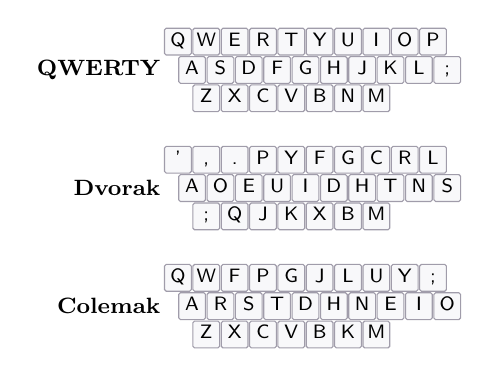
\begin{tikzpicture}
% Three keyboards stacked. Same 30 physical key positions; each layout
% reassigns the letters at those positions. Visual comparison highlights
% how a keymap is a re-binding of an unchanged physical substrate.
% Three keyboards stacked. Punctuation chars are wrapped in {} so
% TikZ's \foreach parser doesn't treat them as separators.
\foreach \layoutY/\name in {3.0/QWERTY, 1.5/Dvorak, 0.0/Colemak} {
 \node[anchor=east, font=\footnotesize\bfseries] at (-0.1, \layoutY+0.36) {\name};
}
% QWERTY rows
\foreach \l [count=\i] in {Q,W,E,R,T,Y,U,I,O,P}
 \node[kcap] at ({(\i-1)*0.36}, 3.72) {\strut\l};
\foreach \l [count=\i] in {A,S,D,F,G,H,J,K,L,{;}}
 \node[kcap] at ({(\i-1)*0.36+0.18}, 3.36) {\strut\l};
\foreach \l [count=\i] in {Z,X,C,V,B,N,M}
 \node[kcap] at ({(\i-1)*0.36+0.36}, 3.0) {\strut\l};
% Dvorak rows
\foreach \l [count=\i] in {{'},{,},{.},P,Y,F,G,C,R,L}
 \node[kcap] at ({(\i-1)*0.36}, 2.22) {\strut\l};
\foreach \l [count=\i] in {A,O,E,U,I,D,H,T,N,S}
 \node[kcap] at ({(\i-1)*0.36+0.18}, 1.86) {\strut\l};
\foreach \l [count=\i] in {{;},Q,J,K,X,B,M}
 \node[kcap] at ({(\i-1)*0.36+0.36}, 1.5) {\strut\l};
% Colemak rows
\foreach \l [count=\i] in {Q,W,F,P,G,J,L,U,Y,{;}}
 \node[kcap] at ({(\i-1)*0.36}, 0.72) {\strut\l};
\foreach \l [count=\i] in {A,R,S,T,D,H,N,E,I,O}
 \node[kcap] at ({(\i-1)*0.36+0.18}, 0.36) {\strut\l};
\foreach \l [count=\i] in {Z,X,C,V,B,K,M}
 \node[kcap] at ({(\i-1)*0.36+0.36}, 0) {\strut\l};
\end{tikzpicture}}
\caption{Tre skrive-tastaturkort over det samme fysiske substrat. Hvert layout er en gen-binding af identiske tastepositioner til et andet sæt bogstaver. QWERTY (Sholes 1873, aldrig patenteret), Dvorak (Dvorak \& Dealey 1936, US 2{,}040{,}248), Colemak (Coleman 2006, public domain). Forgreningsøkosystemet efter 2010 forlænger denne linje.}
\label{fig:typing-layouts}
\end{figure}

\section{Slægtslinje II: instrumentlayouts}
\label{sec:lineage2}

Musikalske instrumentlayouts har gennemløbet en parallel historie. Paul von Jankós seksrækkede isomorfe klaverklaviatur~\citep{janko1882} blev anbefalet af Liszt og Rubinstein, fremstillet af Decker, Blüthner og Bösendorfer, og undervist på et Janko-konservatorium i New York. Ud fra enhver social forudsætning for udbredelse burde det have erstattet det almindelige klaverklaviatur. Det skete ikke. Færre end ti Janko-klaverer vides at have overlevet. Janko-tilfældet er den negative pol i argumentet om tastaturkort-som-social-software: enhver betingelse for udbredelse var opfyldt, og udbredelsen slog alligevel fejl. Hvad social software-kontrakten end er, er den mere end summen af anbefalinger, fabrikanter og konservatorier.

R.\ H.\ M.\ Bosanquets generaliserede klaviatur~\citep{bosanquet1875generalized} var et enharmonisk harmonium med en 53-deling af oktaven (53-EDO) og et orgel fra 1875 i 48-tonet skismatisk og kvartkomma-middeltone, demonstreret for South Kensington Museum i 1876. Det er forfaderen til stort set enhver moderne isomorf controller. Kaspar Wicki patenterede et isomorft nodelayout til bandoneon i 1896~\citep{wicki1896}; Brian Hayden, en koncertina-spiller, genopfandt og genpatenterede uafhængigt stort set det samme layout i 1986. Den dobbelte opfindelse med halvfems års mellemrum er i sig selv et argument: layoutet har karakter af en \emph{opdagelse}, den slags objekt der genopstår, fordi musikkens underliggende struktur gør det nyttigt, ikke fordi det er et unikt kulturelt artefakt.

\begin{figure}[t]
\centering
\resizebox{0.88\columnwidth}{!}{%
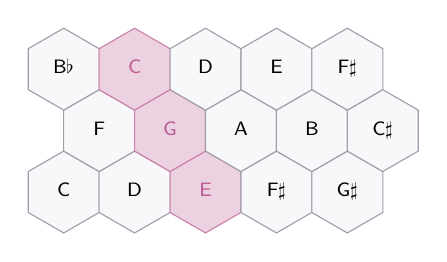
\begin{tikzpicture}
% Compact Wicki-Hayden-style hex schematic. Same-row neighbors
% differ by a whole tone; up-and-right neighbors differ by a P4.
% C major triad (C-E-G) highlighted; the same shape transposes to
% any key by translation across the surface ("isomorphism" claim).
% Hexes are EXPLICIT PATHS, not regular-polygon nodes — TikZ node
% sizing breaks the lattice. Pointy-top hexagon, circumradius R:
% width = sqrt(3)R, height = 2R. Tessellation: horizontal pitch =
% sqrt(3)R, row step = 1.5R, odd-row offset = sqrt(3)R/2.
\def\R{0.52}
\def\hexn#1#2#3{\begin{scope}[shift={(#1,#2)}]
 \draw[keystroke, fill=keyfill]
  (30:\R) -- (90:\R) -- (150:\R) -- (210:\R) -- (270:\R) -- (330:\R) -- cycle;
 \node[font=\scriptsize\sffamily, inner sep=0pt] at (0,0) {\strut#3};
\end{scope}}
\def\hexm#1#2#3{\begin{scope}[shift={(#1,#2)}]
 \draw[keymapped!70, fill=keymapped!25]
  (30:\R) -- (90:\R) -- (150:\R) -- (210:\R) -- (270:\R) -- (330:\R) -- cycle;
 \node[font=\scriptsize\sffamily, text=keymapped!90, inner sep=0pt] at (0,0) {\strut#3};
\end{scope}}
\def\hp{0.9006}  % horizontal pitch (sqrt(3) * R)
\def\vp{0.78}   % vertical pitch (1.5 * R)
\def\offx{0.4503} % horizontal offset for alternate rows (hp / 2)
% Row 0 (bottom)
\hexn{0}{0}{C}
\hexn{\hp}{0}{D}
\hexm{2*\hp}{0}{E}
\hexn{3*\hp}{0}{F$\sharp$}
\hexn{4*\hp}{0}{G$\sharp$}
% Row 1 (middle, offset)
\hexn{\offx}{\vp}{F}
\hexm{\offx + \hp}{\vp}{G}
\hexn{\offx + 2*\hp}{\vp}{A}
\hexn{\offx + 3*\hp}{\vp}{B}
\hexn{\offx + 4*\hp}{\vp}{C$\sharp$}
% Row 2 (top)
\hexn{0}{2*\vp}{B$\flat$}
\hexm{\hp}{2*\vp}{C}
\hexn{2*\hp}{2*\vp}{D}
\hexn{3*\hp}{2*\vp}{E}
\hexn{4*\hp}{2*\vp}{F$\sharp$}
\end{tikzpicture}}
\caption{Wicki--Hayden-hexlayout (Wicki 1896 / Hayden 1986). Naboer i samme række adskiller sig med en heltone; naboer op-og-til-højre med en ren kvart. C-dur-treklangen ($C\,E\,G$) er fremhævet: akkorden er en fast tre-celle-form på overfladen, og at flytte den form transponerer akkorden til enhver toneart. ``Transponering er translation'' er den centrale påstand om isomorfe klaviaturer, og den egenskab, som det almindelige klavers asymmetri mellem hvidt og sort ofrer.}
\label{fig:wicki}
\end{figure}

\begin{figure*}[t]
\centering
% Interval-signature bars (full text width). Each bar reads left to
% right as the sequence of intervals the instrument's layout steps
% through; every block is one interval, its WIDTH = its size in
% semitones and its COLOR fixed by the legend. A regular instrument
% is a row of equal blocks; an asymmetric one has a visible odd block.
\begingroup
\definecolor{iv1}{HTML}{E2574C}% m2 (1 semitone)
\definecolor{iv2}{HTML}{EE9B3A}% M2 (2)
\definecolor{iv3}{HTML}{D1A52A}% m3 (3) — darkened so white slice text reads
\definecolor{iv4}{HTML}{4FAE54}% M3 (4)
\definecolor{iv5}{HTML}{3A86D6}% P4 (5)
\definecolor{iv7}{HTML}{8A5CF6}% P5 (7)
\resizebox{\textwidth}{!}{%
\begin{tikzpicture}
\def\rad{1.55}
% \pie{xshift}{name}{deg-per-semitone}{ semitones/color/label, ... }
% Slices sweep clockwise from 12 o'clock; angle = semitones. A regular
% instrument is an even wheel; an asymmetric one has a visibly odd slice.
% list fields: semitones / fill / interval-label / note-label.
% The note sits INSIDE the slice (the actual open string, scale degree,
% or valve number); the interval name sits just outside the rim.
\def\pie#1#2#3#4{\begin{scope}[shift={(#1,0)}]
 \xdef\angA{90}
 \foreach \s/\c/\lab/\nt in {#4}{
  \pgfmathsetmacro\angB{\angA-\s*#3}
  \filldraw[fill=\c, draw=\c!55!black, line width=0.6pt]
   (0,0) -- (\angA:\rad) arc[start angle=\angA, end angle=\angB, radius=\rad] -- cycle;
  \pgfmathsetmacro\angM{(\angA+\angB)/2}
  \node[font=\large\sffamily\bfseries, text=white] at (\angM:{0.58*\rad}) {\nt};
  \node[font=\small\sffamily, text=acdark] at (\angM:{\rad+0.32}) {\lab};
  \xdef\angA{\angB}
 }
 \node[font=\normalsize\sffamily\bfseries, text=acdark] at (0,{-\rad-1.08}) {#2};
\end{scope}}
% --- legend ---
\begin{scope}[shift={(-0.4,3.15)}]
 \node[font=\small\sffamily\bfseries, text=acdark, anchor=west] at (0,0.28) {Interval \;(udsnitsvinkel $\propto$ halvtoner):};
 \def\lg#1#2#3{\draw[fill=#2, draw=#2!55!black, rounded corners=2pt] (#1,0.0) rectangle (#1+0.56,0.56);
  \node[font=\small\sffamily, text=acdark, anchor=west] at (#1+0.66,0.28) {#3};}
 \lg{7.7}{iv1}{m2}\lg{9.1}{iv2}{M2}\lg{10.5}{iv3}{m3}\lg{11.9}{iv4}{M3}\lg{13.3}{iv5}{P4}\lg{14.7}{iv7}{P5}
\end{scope}
% --- four wheels in a row ---
\pie{0}{Guitar \textperiodcentered\ EADGBE}{15}{5/iv5/P4/E, 5/iv5/P4/A, 5/iv5/P4/D, 4/iv4/M3/G, 5/iv5/P4/B}
% emphasize the guitar's lone M3 wedge (starts -135, spans 60 deg)
\draw[keymapped, line width=1.5pt]
 (0,0) -- (-135:\rad) arc[start angle=-135, end angle=-195, radius=\rad] -- cycle;
\pie{4.7}{Violin \textperiodcentered\ GDAE}{17.142857}{7/iv7/P5/G, 7/iv7/P5/D, 7/iv7/P5/A}
\pie{9.4}{Trumpet \textperiodcentered\ 3 ventiler}{60}{2/iv2/M2/1, 1/iv1/m2/2, 3/iv3/m3/3}
\pie{14.1}{Ocarina \textperiodcentered\ diatonisk}{30}{2/iv2/M2/C, 2/iv2/M2/D, 1/iv1/m2/E, 2/iv2/M2/F, 2/iv2/M2/G, 2/iv2/M2/A, 1/iv1/m2/B}
\end{tikzpicture}}
\endgroup
\caption{Fire asymmetriske tonehøjde-grænseflader læst som \emph{intervalhjul}. Hvert hjul fejer med uret gennem de intervaller, dets layout er bygget af; hvert udsnit er ét interval, dets vinkel sat af dets størrelse i halvtoner og dets farve fastlagt af signaturen. Et regelmæssigt instrument er et jævnt hjul; et asymmetrisk bærer et synligt skævt udsnit. Guitar EADGBE er en ring af rene kvarter brudt én gang af den store terts mellem G og B (optrukket) --- den uregelmæssighed, der lader standard-akkordgrebene ligge under hånden, og som folk-, blues-, jazz- og rockguitar er blevet skrevet imod. Violin er tre identiske rene kvinter: et fuldkommen jævnt hjul, men hver løs streng en anden absolut tonehøjde. Trompetens tre ventiler sænker tonehøjden med to, en og tre halvtoner --- alle forskellige ved design, så deres kombinationer når hvert kromatisk trin. Okarinaen er den diatoniske skalas eget hjul, to korte trin blandt fem lange. Det almindelige klaver hører til samme familie: det diatoniske navngivnings-tastaturkort legemliggjort i mange overflader, hver med sin egen asymmetri.}
\label{fig:asymmetric-instruments}
\end{figure*}

Hver af disse overflader bærer sin egen slægtshistorie. Den treventilede trompet (Stölzel og Blühmel, ca.\ 1814) standardiserede efter et århundredes naturtrompetpraksis, med Wiener- og rotationsventil-varianter, der hver udgør sit eget tastaturkort-over-tonehøjde. Okarinaen løber fra mesoamerikanske karfløjter gennem Giuseppe Donatis standardisering i 1853 i Budrio, hvor asymmetrisk placering af fingerhuller gjorde 10-hulsmønstret undervisbart. Guitarens EADGBE-stemning krystalliserede i 1700-tallet ud af lutstemninger: B-strengens uregelmæssighed bryder de ellers ensartede kvarter, så de åbne akkordgreb ligger under hånden, og hele litteraturen af folk-, blues-, jazz- og rockguitar er blevet skrevet imod det ene uregelmæssige interval. Violinens strenge rene kvinter (G\,D\,A\,E) forankrer de kvint-baserede strygerkonventioner, som det orkestrale repertoire er skrevet ind i. I hvert tilfælde er asymmetrien ikke en fejl, musikken tolererer, men en arv, musikken er blevet skrevet omkring --- den afgør, hvad en begynder lærer først, hvordan en øveøvelse ser ud, hvilken notation der rejste. Det almindelige klaverklaviatur sidder inde i denne tradition, ikke over den; de isomorfe alternativer foreslår noget mere radikalt, end de undertiden indrømmer, nemlig opløsningen af det tastaturkort-over-tonehøjde-navngivning, der forbinder alle disse instrumentfamilier med hinanden.

Den gængse læsning af Jankós fiasko --- og af Wicki--Hayden-/hex-gitter-familiens marginalitet mere generelt --- er stiafhængighed efter David--Liebowitz-modellen: klaveret består alene ved lock-in. En hårdere læsning er tilgængelig. Det almindelige klaverklaviaturs asymmetri mellem hvidt og sort er et landemærke-kort over den kromatiske cirkel --- spilleren ved, hvor $C$ er, fordi det sidder til venstre for to sorte --- og aflaster absolut tonehøjdeposition fra hukommelsen over på øjet og hånden. Fjern asymmetrien, og den aflastede information har intetsteds at lande: transponering bliver translation, men absolut placering bliver erindring. Fire århundreders repertoire har optaget asymmetrien i \emph{tonearts-karakter} --- fingersætningen i $F^\sharp$-dur adskiller sig fra den i $C$-dur, og musikken er skrevet til den forskel --- så at fjerne ``historiens tilfældighed'' fladgør en betydningsakse, litteraturen er blevet skrevet langs med. Dette opløser ikke så meget stiafhængighedsfortællingen, som det skærer langs den fra den anden side: klaveret er stiafhængigt \emph{og} stien har frembragt et objekt, der ikke er strengt ækvivalent med sine alternativer. Det dybere træk er at behandle selve det vestlige tonale system som et tastaturkort: den syvbogstavs diatoniske navngivning $C\,D\,E\,F\,G\,A\,B$ er allerede en social software-kontrakt over tonehøjderummet, indskrevet i teori, pædagogik og enhver toneartsangivelse. Klaverets hvide tangenter er den fysiske realisering af det tastaturkort; de sorte tangenter er de ændringer, notationen allerede navngiver med $\sharp$ og $\flat$. Det almindelige klaver udfører således to opgaver på én gang --- fysisk grænseflade og notationskodning --- og de isomorfe alternativer foreslår at opløse den anden for at optimere den første. Argumentet er afgrænset til det 12-tone-ligesvævende repertoire, der navngiver tonehøjder med de diatoniske bogstaver; uden for det --- xenharmonisk musik i 19-, 22-, 31-, 53-EDO, maqam og andre tonale systemer med andre tonehøjde-navngivnings-tastaturkort --- er klaveret aktivt obstruerende, og den isomorfe linje fra Bosanquet gennem Lumatone har en stærk, repertoire-forankret påstand. Inden for det afgrænsede er det samme tastaturkort-over-tonehøjde-navngivning det, som \texttt{notepat.com} (\textsection\ref{sec:notepat}) bevarer, båret over på QWERTY's bogstavtangenter, hvor det at trykke på bogstavet \texttt{C} spiller noden $C$. Hvor Jankó opløser navngivnings-tastaturkortet for at optimere den fysiske grænseflade, og DAW-konventionen med den kromatiske trappe opløser \emph{begge} (\textsection\ref{sec:daw}), holder \texttt{notepat.com} navngivningskontrakten uændret og stiller kun på ny det spørgsmål, Sholes' mekanikere stillede i 1873: hvilken fysisk overflade bør bære den videre.

De samtidige efterkommere er kommercielle produkter: C-Thru AXiS-49 (2008)~\citep{cthru2008axis49}, Jim Plamondons Thummer~\citep{plamondon2003thummer}, Roger Linns LinnStrument, ROLI Seaboard, Lumatones hex-gitter og Lippold Hakens Continuum Fingerboard~\citep{haken1998indiscrete}. Andrew Milne, William Sethares og James Plamondons artikler om isomorfe controllere og stemnings-kontinua~\citep{milne2007isomorphic,milne2008tuning} leverer det teoretiske fundament. Hvad der er slående fra et tastaturkort-som-social-software-synspunkt er, at disse instrumenter \emph{leveres konfigurerbare}: layoutet er et eksplicit objekt, brugeren uploader, og det xenharmoniske fællesskab deler layouts som filer. Lumatone behandler især tastaturkortet som distributionsenheden. Instrumentet er et substrat; tastaturkortet er det artefakt, der gør det musikalsk.

\section{Den kromatiske trappe, eller AWSED: konvergens uden ejerskab}
\label{sec:daw}

Det stærkeste samtidige tilfælde for argumentet om tastaturkort-som-social-software er det de facto kromatiske QWERTY-klaver-trappekort, som ethvert større digitalt lydværksted deler. Ableton Live, Logic Pro, GarageBand og FL Studio leverer alle den samme konvention som standard~\citep{ableton_musical_typing,apple_logic_musicaltyping,imageline_typing_piano}. Konventionens form er: tag de tre nederste rækker af QWERTY-tastaturet; behandl én række som de hvide tangenter på en kromatisk skala, opstigende fra C; og behandl rækken ovenfor som de sorte tangenter, i de mellemrum hvor sorte tangenter ville falde på et klaver. Ableton, Logic og GarageBand bruger \keys{A,S,D,F,G,H,J,K} (grundrækken) til de hvide tangenter $C\,D\,E\,F\,G\,A\,B\,C$ og \keys{W,E,T,Y,U} (rækken ovenfor) til de sorte tangenter $C^\sharp\,D^\sharp\,F^\sharp\,G^\sharp\,A^\sharp$. FL Studio bruger den nederste række \keys{Z,X,C,V,B,N,M} til den nedre oktavs hvide tangenter og det samme mønster i rækken ovenfor til de sorte tangenter. Princippet er identisk. Den nøjagtige række-tildeling adskiller sig med én række.

Denne konvention har udbredt sig i tre årtier uden et navn. Jeg navngiver den her, for det felt, der burde studere den: læs tangenterne for de fem første kromatiske toner --- $C$ på \key{A}, $C^\sharp$ på \key{W}, $D$ på \key{S}, $D^\sharp$ på \key{E}, $E$ på \key{D} --- i tonehøjderækkefølge, og de staver \textbf{AWSED}. \emph{Herefter AWSED-layoutet} (grundrække-varianten; FL Studio-varianten er dens transposition til den nederste række). Navnet er valgt, så det rimer på WASD, PC-gamingens bevægelseskonvention, der drøftes nedenfor: de to er strukturelt det samme objekt --- et herreløst, uspecificeret, applikationsovergribende input-tastaturkort, som ingen designede og alle leverer --- og rimet er argumentet. WASD blev navngivet, undervist og kanoniseret af sit fællesskab; AWSED blev aldrig engang navngivet, hvilket er præcis grunden til, at den er undsluppet studium. En ting uden et navn er svær at se, sværere at kritisere og umulig at citere. At navngive den er det første træk.

Ingen designede denne konvention. Ingen specifikation definerer den. Der er intet styrende organ, ingen vedligeholder, ingen finansieringsmekanisme. Konventionen eksisterer, fordi de fire implementeringer er enige, og de fire implementeringer er enige, fordi konventionen allerede var til stede i 1990'ernes tracker-software, der gik forud for det moderne DAW (FastTracker, Renoise, Impulse Tracker), og fordi enhver bruger, der har lært ét DAW, forventer, at det næste opfører sig på samme måde. Tutorial-dokumentation skrevet til ét DAW overføres, mere eller mindre, til et andet. Dette er \emph{social software-kontrakten} i sin reneste form: et versioneret virtuelt objekt, der udbreder sig gennem pædagogik og forventning, uden nogen central myndighed.

\begin{figure}[t]
\centering
\resizebox{\columnwidth}{!}{%
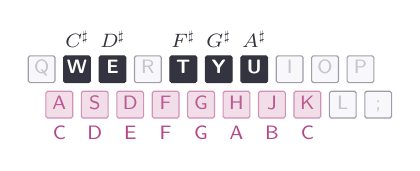
\begin{tikzpicture}
% Upper QWERTY row (sharps in DAW chromatic-staircase). Only 5 keys
% are mapped (W E T Y U); R and I sit in the gaps with no note.
\foreach \l/\note/\mapped [count=\i] in {%
 Q/{}/0, W/$C^\sharp$/1, E/$D^\sharp$/1, R/{}/0, T/$F^\sharp$/1,
 Y/$G^\sharp$/1, U/$A^\sharp$/1, I/{}/0, O/{}/0, P/{}/0%
}{
 \ifnum\mapped=1
  \node[kcap sharp] (k\i) at ({(\i-1)*0.45}, 1.8) {\strut\l};
  \node[font=\scriptsize\sffamily, text=keysharp, anchor=south, inner sep=1pt]
   at ({(\i-1)*0.45}, 2.03) {\note};
 \else
  \node[kcap, text=keystroke!60] (k\i) at ({(\i-1)*0.45}, 1.8) {\strut\l};
 \fi
}
% Home row (whites). 8 of 10 keys mapped (A through K = C..C).
\foreach \l/\note/\mapped [count=\i] in {%
 A/C/1, S/D/1, D/E/1, F/F/1, G/G/1, H/A/1, J/B/1, K/C/1, L/{}/0, {;}/{}/0%
}{
 \ifnum\mapped=1
  \node[kcap mapped] at ({(\i-1)*0.45+0.225}, 1.35) {\strut\l};
  \node[font=\scriptsize\sffamily, text=keymapped, anchor=north, inner sep=1pt]
   at ({(\i-1)*0.45+0.225}, 1.12) {\note};
 \else
  \node[kcap, text=keystroke!60] at ({(\i-1)*0.45+0.225}, 1.35) {\strut\l};
 \fi
}
\end{tikzpicture}}
\caption{AWSED-layoutet --- DAW'ens kromatiske QWERTY-klaver-trappekort (Ableton-, Logic-, GarageBand-varianten). Grundrækken \texttt{A~S~D~F~G~H~J~K} spiller de hvide tangenter $C$ til $C$; rækken ovenfor placerer krydsene i de mellemrum, hvor klaverets sorte tangenter ville falde ($C^\sharp\,D^\sharp$ derefter et mellemrum ved \texttt{R}, $F^\sharp\,G^\sharp\,A^\sharp$, derefter mellemrum). Navnet kommer fra de fem første kromatiske toner $C\,C^\sharp\,D\,D^\sharp\,E$, som falder på \key{A}\,\key{W}\,\key{S}\,\key{E}\,\key{D}. QWERTY-bogstavet på hver tangent har ingen relation til det nodenavn, det frembringer.}
\label{fig:daw-staircase}
\end{figure}

Det er også, vil jeg argumentere for, dårligt designet. AWSED-layoutet har tre strukturelle svagheder. \textbf{For det første} har QWERTY-bogstavet på hver tast ingen relation til det nodenavn, det frembringer. \key{A} spiller C; \key{S} spiller D; \key{D} spiller E (Figur~\ref{fig:daw-staircase}). En bruger, der har lært den vestlige syvtones skala, opnår ingen greb om tastaturkortet ud fra den viden. \textbf{For det andet} leverer det kun en enkelt oktav ($C$ til $C$), men spreder den ene oktav helt hen over grundrækken, fra \key{A} til \key{K} --- den fulde bredde, hvor \emph{begge} hænder hviler. Det er hverken en kompakt enhånds-oktav eller et produktivt tohånds-omfang: det bruger to hænders værd af tastatur til at frembringe en enkelt oktav og stopper der. Bredden er lagt ud som til to hænder, men omfanget er dimensioneret til én. \textbf{For det tredje} er tastaturkortet ulæseligt uden en tutorial: der er ingen huskeregel, intet diagram trykt på de fysiske taster, og ingen måde at udlede kortlægningen fra første principper. Et tastaturkort, der kræver en manual, er et tastaturkort, der har mistet sin social software-karakter.

Navngivningen var ikke tilfældig. Dens naturlige modstykke er WASD, bevægelseskonventionen i PC-gaming --- og det nære anagram er ikke så meget et tilfælde som en diagnose. WASD har den samme strukturelle form som AWSED --- en herreløs, uspecificeret, applikationsovergribende bruger-input-konvention --- men en anden udbredelseshistorie. Før WASD brugte PC-spil som standard piletasterne (Wolfenstein 3D, Doom, Quake-serien frem til 1997)~\citep{wikipedia_arrow_keys}; mellemliggende eksperimenter omfattede System Shocks ASDX (1994) og Descents AZ+QE. Dennis ``Thresh'' Fong, en konkurrencespillende Quake-spiller, populariserede WASD-layoutet gennem sin selvudgivne konfigurationsguide~\citep{thresh_quake_bible} og vandt det første landsdækkende Quake-mesterskab i 1997. Valves Half-Life leverede WASD som standard i 1998, og i begyndelsen af 2000-tallet havde konventionen mættet PC-spillene~\citep{fenlon2016wasd}. WASD består af en grund, som DAW'ens kromatiske trappe ikke har: den er reelt bedre end den officielle standard. Den frigør højre hånd til musen, sidder ved siden af Shift / Space / Ctrl / Tab og udnytter grundrækkens fingerplacering på et QWERTY-tastatur. Den strukturelle lektie er, at udbredelse er en funktion af social mediering \emph{og} egnethed: WASD udbredte sig, fordi Fongs pædagogik nåede spillerne \emph{og} kortlægningen vandt på sine fortjenester. Den kromatiske trappe udbredte sig gennem pædagogik alene, til trods for at fortjenesterne løber den anden vej. Begge tilfælde sidder i samme kategori --- herreløse konventioner, der styrer bruger-input på tværs af applikationer. De viser, at kategorien er stor nok til at spænde over både det veldesignede og det dårligt designede, det bruger-validerede og det arvet-ved-inerti.

\section{Notepat.com: noder der navngiver sig selv}
\label{sec:notepat}

Mod denne etablerede foreslår \texttt{notepat.com} et andet tastaturkort (Figur~\ref{fig:notepat-keymap}). Designprincippet er enkelt: \emph{noder der navngiver sig selv}. QWERTY-bogstavet \key{C} spiller C. QWERTY-bogstavet \key{D} spiller D. Den vestlige skalas syv stamtoner --- $C\,D\,E\,F\,G\,A\,B$ --- spiller de noder, deres bogstaver navngiver. Den øvre oktav fortsætter alfabetisk: \keys{H,I,J,K,L,M,N} for $C_5\,D_5\,E_5\,F_5\,G_5\,A_5\,B_5$. Krydsene sidder én række over deres stamtone, i analogi med klaverets sorte tangenter, hvor QWERTY-bogstaverne tillader det: \keys{V,S,W,R,Q} for $C^\sharp\,D^\sharp\,F^\sharp\,G^\sharp\,A^\sharp$. Den nedre oktav falder under venstre hånd; den øvre oktav falder under højre.

Tastaturkortet vender hver af AWSED's tre svagheder om. \textbf{For det første} \emph{er} bogstavet på hver tast nodenavnet. Enhver, der kender den vestlige skala, kender allerede tastaturkortet. \textbf{For det andet} bruger det tohånds-bredden produktivt: venstre hånd spiller den nedre oktav, og højre hånd spejler den på den øvre, så det samme spænd, AWSED bruger på en enkelt oktav, giver to. \textbf{For det tredje} er tastaturkortet selvdokumenterende: diagrammet i Figur~\ref{fig:notepat-keymap} kan gengives fra hukommelsen af enhver, der kan stave ``CDEFGAB.''

Tre ting gør \texttt{notepat.com} usædvanlig blandt denne artikels tastaturkort: det har et navn --- de fleste, som AWSED (\textsection\ref{sec:daw}), fik aldrig ét --- dets noder navngiver sig selv, så tastaturkortet adresserer sig selv, og det kører allerede i mange implementeringer. \texttt{notepat.com}'s bidrag er ikke implementeringen. Implementeringen er, ved design, beskeden: et par hundrede linjers JavaScript, der dirigerer tastaturhændelser til en lydsyntese-API. Bidraget er tastaturkortet. Det fremlægges på tværs af fem implementeringer --- web-stykket på \texttt{notepat.com}, bare-metal-porten til AC Native OS, MenuBand-appen i macOS-menulinjen, Ableton-pluginet (Max for Live) og \texttt{babypat} --- og tastaturkortet er den ene ting, der er identisk på tværs af dem alle. Node-navngivnings-notationen rejser endnu længere end instrumentet: den genbruges i \texttt{clock}, AC's distribuerede sequencer, hvor de samme étbogstavs tonehøjder driver netværksbaseret afspilning. Det er den \texttt{notepat.com}-formede social software-kontrakt.

En læser, der sammenligner implementeringerne side om side, vil bemærke taster, der gør ting ud over tabellen i Figur~\ref{fig:notepat-keymap}. På AC Native og MenuBand afspiller det at holde \texttt{Space} de sidste par sekunder af det faktiske lydoutput baglæns. På web-stykket og AC Native giver det at holde \texttt{Shift}, mens man slår en node an, den stemme en lang udklingshale, når den slippes; det at holde \texttt{Enter} holder stemmen i det uendelige, og \texttt{Backspace} rydder hver holdt stemme. På MenuBand og AC Native forfremmer \texttt{Control}, \texttt{Alt} og de to sammen et enkelt tastetryk til en dur-, mol- eller forholds-treklang. Intet af dette fremgår af tastaturkort-diagrammet, og udeladelsen er bevidst. Disse bindinger danner et \emph{udvidet performance-lag}, og grænsen mellem det lag og den tonale kortlægning er selve grænsen for social software-kontrakten (Tabel~\ref{tab:contract-line}).

\begin{table}[t]
\footnotesize
\setlength{\tabcolsep}{3pt}
\renewcommand{\arraystretch}{1.05}
\centering
\caption{Bindingerne i \texttt{notepat.com}, delt ved kontraktlinjen. Over linjen: den tonale kortlægning, identisk på tværs af alle implementeringer --- social software-objektet. Under den: det udvidede performance-lag, hvor hvert substrat frit kan afvige.}
\label{tab:contract-line}
\begin{adjustbox}{max width=\linewidth,center}%
\begin{tabularx}{\linewidth}{@{}>{\RaggedRight}p{0.30\columnwidth}>{\RaggedRight}X>{\RaggedRight\arraybackslash}p{0.21\columnwidth}@{}}
\toprule
\textbf{Binding} & \textbf{Betydning} & \textbf{Hvor} \\
\midrule
\multicolumn{3}{@{}l}{\emph{Tonal kontrakt}} \\[0.1em]
\texttt{C D E F G A B} & stamtoner $C_4$--$B_4$, venstre hånd & alle \\
\texttt{H I J K L M N} & stamtoner $C_5$--$B_5$, højre hånd & alle \\
\texttt{V S W R Q} & krydser, én række over & alle \\
\midrule
\multicolumn{3}{@{}l}{\emph{Udvidet performance-lag}} \\[0.1em]
\texttt{Shift} (hold) & sustain: lang udklingshale & web, Native \\
\texttt{Enter} (hold) & hold stemme; \texttt{Backspace} rydder & web, Native \\
\texttt{Space} (hold) & afspil nylig lyd baglæns & Native, MenuBand \\
\texttt{Ctrl}\,/\,\texttt{Alt}\,/\,begge & dur\,/\,mol\,/\,sus2-treklang & MenuBand, Native \\
\texttt{<}~\texttt{>} & oktavskift pr.\ hånd & web \\
\bottomrule
\end{tabularx}%
\end{adjustbox}
\end{table}

De to halvdele af Tabel~\ref{tab:contract-line} styres af forskellige regler. Over linjen er afvigelse brud: en implementering, der omkortlagde \texttt{C} væk fra noden $C$, ville ikke være en \texttt{notepat.com}-port, men et andet instrument. Under linjen er afvigelse idiom: hvert substrat dyrker de gestus, dets krop muliggør. Bare-metal-OS'et, der ejer hele maskinen, kan ringbuffere sit eget lydoutput og afspille det baglæns; menulinje-appen, der rider på en systemdækkende event tap, læner sig op ad modifikator-akkorder; web-stykket, der lever i en browserfane, holder og lader klinge. Brugerne oplever ikke disse forskelle som brud, og ingen implementering er forpligtet til at bære en andens gestus. Den samme to-lags-struktur er synlig i de ældre tilfælde: QWERTY-kontrakten siger intet om medietaster eller \texttt{Fn}-lag, der varierer frit fra producent til producent, uden at nogen kalder en ThinkPad en forgrening af QWERTY; Vims kernebevægelser er kontrakt, mens plugin-bindinger er idiom. Et tastaturkort, antyder dette, er ikke mængden af alle bindinger, en implementering leverer. Det er den delmængde, hvis ændring fællesskabet ville opleve som et brud på identiteten --- og en praktisk test for, hvilken side af linjen en binding falder på, er, om notationsoverfladen (\textsection\ref{sec:notation}) bærer den. \texttt{C D E F G A B} rejser som tekst; ``hold mellemrum for at vende tiden'' er en substrat-specifik gestus, der må genlæres, ved demonstration, ved enhver port.

Dette er det træk, artiklen beder læseren om at se. Det dominerende DAW-kromatiske-trappekort blev aldrig \emph{valgt} --- det blev \emph{arvet} fra tracker-software, opretholdt af brugerforventning og låst fast af applikationsovergribende konvention. \texttt{notepat.com} demonstrerer, at hullet er åbent: at et bevidst designet alternativ kan forfattes af en enkelt udvikler på et par hundrede linjers kode, leveres på tværs af flere implementeringer i løbet af et år og tilbydes et bredere fællesskab som en konkurrerende social software-kontrakt. Den politiske indsats er lille i ethvert enkelt tilfælde og stor i sin helhed: \emph{hullet er åbent overalt}.

\section{Notation: den diskursive overflade}
\label{sec:notation}

Argumentet hidtil har behandlet tastaturkortet som en tabel. Men et tastaturkort er ikke kun en tabel. Det har også en \emph{notation} --- en tekstlig form, hvori brugen af tastaturkortet læses, skrives, undervises, citeres og diskuteres. Notationen er tastaturkortets diskursive overflade. Den er også, vil jeg argumentere for, den halvdel af tastaturkortet, der faktisk rejser. Et tastaturkort, hvis notation er portabel, udbreder sig som tekst; et tastaturkort, hvis notation er kluntet eller fraværende, udbreder sig kun som muskelhukommelse. Notationens kvalitet er derfor en designbar egenskab ved tastaturkortet, ikke et afledt artefakt. En designer, der kun leverer bindingstabellen, har leveret halvdelen af objektet.

Det kanoniske tilfælde er Vim. Vims underliggende tastaturkort er en tabel, der kortlægger tastetryk til editor-kommandoer: \texttt{d} indleder en sletteoperator, \texttt{i} et indre tekstobjekt, \texttt{w} en ordbevægelse. Hvad der rejser i Vim-diskursen, er imidlertid ikke tabellen. Hvad der rejser, er en \emph{notation}: \texttt{dd}, \texttt{ciw}, \texttt{gg}, \texttt{:wq}, \texttt{<C-w>} (Figur~\ref{fig:vim-modes}). Tutorials, blogindlæg, README-filer, vimtutor og den langvarige vim-mod-emacs-diskussion føres alle i denne notation. Notationen er så portabel, at den overlever helt uden for Vim: \emph{vim-tilstand} optræder i Visual Studio Code, i JupyterLab, i shells via \texttt{set -o vi}, i macOS' Cocoa-tekstfelter, i browsere via Vimium. Det, der porteres, er notationen. Runtime er tilfældig.

\begin{figure}[t]
\centering
\begin{tikzpicture}[
 modebox/.style={draw=keymapped!70, fill=keymapped!12,
          rounded corners=2pt, minimum width=1.6cm,
          minimum height=0.6cm, font=\small\sffamily,
          text=keymapped!90, inner sep=2pt},
 arrow/.style={-{Stealth[length=4pt,width=4pt]}, draw=keystroke!90,
         line width=0.5pt},
 cmd/.style={font=\footnotesize\ttfamily, text=acdark}
]
% Three Vim modes wired by their command-notation transitions.
\node[modebox] (normal) at (0, 0) {NORMAL};
\node[modebox] (insert) at (3.0, 0) {INSERT};
\node[modebox] (visual) at (-3.0, 0) {VISUAL};
\draw[arrow] ([yshift=4pt]normal.east) -- node[above, cmd] {\texttt{i}\,/\,\texttt{a}\,/\,\texttt{o}} ([yshift=4pt]insert.west);
\draw[arrow] ([yshift=-4pt]insert.west) -- node[below, cmd] {\texttt{<Esc>}} ([yshift=-4pt]normal.east);
\draw[arrow] ([yshift=4pt]normal.west) -- node[above, cmd] {\texttt{v}\,/\,\texttt{V}\,/\,\texttt{<C-v>}} ([yshift=4pt]visual.east);
\draw[arrow] ([yshift=-4pt]visual.east) -- node[below, cmd] {\texttt{<Esc>}} ([yshift=-4pt]normal.west);
% A row of canonical commands underneath
\node[font=\footnotesize\ttfamily, text=acdark, anchor=north] at (0, -1.0)
 {\texttt{dd}\,\,\texttt{ciw}\,\,\texttt{gg}\,\,\texttt{:wq}\,\,\texttt{<C-w>v}\,\,\texttt{y2}\$};
\end{tikzpicture}
\caption{Vims modale tastaturkort og dets rejsende notation. Tilstande (NORMAL, INSERT, VISUAL) forbindes af mærkede tastetryks-overgange; almindelige kommandoer (\texttt{dd} slet-linje, \texttt{ciw} ændr-indre-ord, \texttt{gg} gå-til-top, \texttt{:wq} skriv-og-afslut osv.) er tastaturkortets diskursive valuta. Notationen er så portabel, at den er blevet genimplementeret i VS~Code, JupyterLab, Vimium, macOS' Cocoa-tekstsystem og \texttt{set -o vi}.}
\label{fig:vim-modes}
\end{figure}

DAW'ens kromatiske trappe er det negative tilfælde. Der findes ingen portabel notation for den. At skrive en melodi spillet på Abletons musical typing kræver, at man falder tilbage på hændelses-sekvens-prosa --- ``tryk på \key{A}, så \key{S}, så \key{D}'' --- der beskriver input snarere end musik. Sammenlign med Singmaster-terningnotationen~\citep{singmaster1981notes} (Figur~\ref{fig:singmaster}), hvor \texttt{R U R' U' R U2 R'} lader en Rubiks-terning-algoritme rejse intakt mellem terningløsere; eller med Nashville Number System~\citep{matthews1984nashville,williams1988nashville}, hvor ``1--4--5'' lader en akkordprogression rejse mellem studiemusikere; eller med Plover-stenografiteorien~\citep{knight2010plover}, hvor akkordnotationen lader stenografiske mønstre rejse gennem en fællesskabsredigeret ordbog. DAW-trappen har intet sådant håndtag. Dens taster kan kun adresseres ved deres fysiske position. Tastaturkortet eksisterer derfor i muskelhukommelsen og sjældent på papiret --- hvilket er præcis grunden til, at det har lavere diskursiv tilstedeværelse end Vim på trods af en formodentlig større brugerbase.

\begin{figure}[t]
\centering
\resizebox{0.62\columnwidth}{!}{%
\begin{tikzpicture}
% Symmetric bounding box around the cube body (x=0) so \centering
% lands it centered --- the quarter-turn arrow otherwise extends the
% natural box rightward and pulls the cube off-center.
\useasboundingbox (-1.85,-2.55) rectangle (1.85,1.55);
% Isometric Rubik's cube, three visible faces: U (top), F (front-
% left), R (right). Faces are explicit-path parallelogram grids built
% from iso axes er=(0.866,0.5)s (right-up), el=(-0.866,0.5)s
% (left-up), ed=(0,-1)s (down), all meeting at the shared front-top
% vertex at the origin. The R face is tinted with a quarter-turn
% arrow: the diagram shows the first move of the algorithm below.
\def\s{0.55}
% Top face U: cells spanned by er and el
\foreach \i in {0,1,2} \foreach \j in {0,1,2}
 \draw[keystroke, fill=keyfill]
  ({0.866*\s*(\i-\j)}, {0.5*\s*(\i+\j)})
  -- ++({0.866*\s}, {0.5*\s})
  -- ++({-0.866*\s}, {0.5*\s})
  -- ++({-0.866*\s}, {-0.5*\s}) -- cycle;
% Front-left face F: cells spanned by el and ed — green stickers
\foreach \i in {0,1,2} \foreach \j in {0,1,2}
 \draw[acgreen!75!black, fill=acgreen!55]
  ({-0.866*\s*\i}, {0.5*\s*\i - \s*\j})
  -- ++({-0.866*\s}, {0.5*\s})
  -- ++(0, {-\s})
  -- ++({0.866*\s}, {-0.5*\s}) -- cycle;
% Right face R: cells spanned by er and ed — red stickers (mid-turn)
\foreach \i in {0,1,2} \foreach \j in {0,1,2}
 \draw[red!70!black, fill=red!55]
  ({0.866*\s*\i}, {0.5*\s*\i - \s*\j})
  -- ++({0.866*\s}, {0.5*\s})
  -- ++(0, {-\s})
  -- ++({-0.866*\s}, {-0.5*\s}) -- cycle;
% Face labels at face centers — standard sticker scheme:
% white up, green front, red right.
\node[font=\small\sffamily\bfseries, text=acdark]
 at (0, {1.5*\s + 0.5*\s}) {U};
\node[font=\small\sffamily\bfseries, text=white]
 at ({-0.866*\s*1.5 - 0.433*\s}, {0.75*\s - 1.5*\s + 0.25*\s}) {F};
\node[font=\small\sffamily\bfseries, text=white]
 at ({0.866*\s*1.5 + 0.433*\s}, {0.75*\s - 1.5*\s + 0.25*\s}) {R};
% Quarter-turn arrow for R: curved arrow hugging the right face's
% outer edge, pointing upward (clockwise as seen from the right).
\draw[-{Stealth[length=5pt,width=5pt]}, line width=1.1pt, red!70!black]
 ({0.866*\s*3.45}, {0.5*\s*3.45 - 2.5*\s})
 to[bend right=42]
 ({0.866*\s*3.45}, {0.5*\s*3.45 - 0.35*\s});
% Notation row underneath
\node[font=\small\ttfamily, anchor=north, text=acdark]
 at (0, {-3.2*\s}) {R\,U\,R$'$\,U$'$\,R\,U2\,R$'$};
\node[font=\scriptsize\sffamily, anchor=north, text=keystroke]
 at (0, {-4.0*\s}) {en algoritme på 7 træk};
\end{tikzpicture}}
\caption{Singmasters terningnotation~\citep{singmaster1981notes}. Hvert stort bogstav navngiver en side (\textsf{U}p, \textsf{D}own, \textsf{L}eft, \textsf{R}ight, \textsf{F}ront, \textsf{B}ack); et nøgent bogstav er en kvartdrejning med uret, et bogstav med mærke ($\,'$) en kvartdrejning mod uret, og et 2-tal en halvdrejning. Den syv-tegns streng \texttt{R U R$'$ U$'$ R U2 R$'$} er en komplet algoritme, der er portabel mellem terningløsere, GitHub-repos og YouTube-tutorials --- parret af tastaturkort og notation, der rejser som tekst. Siderne bærer standard-klistermærke-skemaet (hvid op, grøn front, rød højre); \textsf{R} er tegnet midt i en kvartdrejning: algoritmens første træk.}
\label{fig:singmaster}
\end{figure}

\texttt{notepat.com}'s ``noder-navngiver-sig-selv''-design har, som en strukturel sidevirkning, en notation, der intet koster at lære. For at skrive en notepat.com-sekvens skriver man \texttt{C D E F G A B} --- hvilket også er standard musiknotation. Notationen er ikke opfundet til \texttt{notepat.com}; den er \emph{arvet} fra en eksisterende læsefærdighed. En pianist, der aldrig har set et notepat.com-tastaturkort, kan læse et notepat.com-partitur; omvendt øver en notepat.com-udøver, der lærer tastaturkortet, også standard tonehøjde-bogstav-læsefærdighed. Dette er, hvordan en veldesignet notationsoverflade ser ud: notationen er så trivielt udledelig fra forhåndsviden, at det intet koster at lære den. Abletons kromatiske trappe ville derimod kræve, at et notepat-lignende partitur blev omkodet til \texttt{A S D F G H J} --- en privat notation bundet til ét tastaturkort, ubrugelig andre steder.

Den empiriske litteratur om udbredelse af tastaturgenveje understøtter denne læsning. Peres et al.\ fandt, at det at arbejde sammen med andre genvejsbrugere er en stærkere forudsigelse for genvejsbrug end computererfaring alene~\citep{peres2004shortcut}. Lozhkina et al.\ udvider resultatet: opdagelseskanalen for genveje er interpersonel og visuel~\citep{lozhkina2025discovery}. Wang et al.\ bruger eksplicit termen \emph{vokabular} til at navngive det, genvejsdesign rækker brugeren~\citep{wang2020keymap}. Denne artikels argument skærper disse fund: den sociale mediering er ikke en generisk effekt af at være-omkring-andre-brugere; det er en specifik transmission via notationsoverfladen. Kolleger læser hinandens skærme, ser \texttt{:wq}, spørger, lærer. Hvor der ikke er nogen overførbar notation, er der ingen social mediering at mediere. Den samme logik forklarer succesen for live-codingens mini-notationer: Alex McLean og Geraint Wiggins' mønstersprog TidalCycles~\citep{mclean2010tidal}, porteret til JavaScript som Strudel~\citep{roos2023strudel}, og Olivia Jacks Hydra-transformationskæder til live-kodede visuals~\citep{jack2018hydra}, ved siden af ABC-notation til folkemusik~\citep{walshaw_abc}. I hvert tilfælde er runtime tilfældig --- Haskell, JavaScript, WebGL, MIDI-afspillere --- men notationen bærer praksissen på tværs af runtimes, workshops og årtier.

Følgesætnings-kataloget i \textsection\ref{sec:corollaries} er, læst gennem denne linse, næsten udelukkende et katalog af notationer. Singmaster, Nashville, ABC, IPA, Camelot, fightingspillenes numpad-notation, videnskabelig tonehøjde, NATO-staveafabetet, strikkeforkortelser --- hver er en notation afledt af et tastaturkort (eller en inputkortlægning), der lod den underliggende praksis rejse som tekst. Parret af tastaturkort og notation er enheden. Tastaturkortet leverer affordancen; notationen leverer udbredelsesoverfladen.

Den strukturelle påstand har en dybere diagnose. Walter Ongs sondring mellem oralitet og litteracitet~\citep{ong1982orality}, der bygger på Havelocks redegørelse for den samme overgang i det antikke Grækenland~\citep{havelock1963preface}, skærer spørgsmålet rent over. \emph{Orale} traditioner består gennem performance, person-til-person-transmission og gentagen tilnærmelse; de har ingen kanonisk tekst, muterer en smule fra instans til instans og overlever, fordi udøvere bliver ved med at udøve dem. \emph{Litterate} traditioner består gennem fast tekst, autoritative udgaver og nøjagtig reproduktion; de har specifikationer, kanoner og referenceimplementeringer. Datalogiens standardrammer er alle litterate rammer: en open source-licens styrer en fast tekst, en protokol styrer et fast wire-format, et format styrer en fast kodning. DAW'ens kromatiske trappe er et primært-oralt tastaturkort --- der er ingen kanonisk tekst, kun fire implementeringer, der er enige ved performance. Vim har både et oralt substrat (man lærer tastaturkortet ved at se en anden udviklers skærm) og en litterat kant (notationen: \texttt{:wq}, \texttt{<C-w>}, \texttt{ciw}). \texttt{notepat.com} kollapser den litterate side ind i den bestående læsefærdighed for tonehøjde-bogstav-notation: tastaturkortet arver sin skrevne form fra en flere århundreder ældre litterat praksis. Det orale substrat er tastaturkortet; notationen er den litterate fiksering; hvor sidstnævnte lykkes, får førstnævnte et legeme, der rejser. Oralitets-litteracitets-aksen er diagnosen på, hvorfor tastaturkort overhovedet undslipper open source-/proprietær-rammen: standardrammerne er litterate rammer, men tastaturkortet er i det mindste delvis oralt, og fraværet af en litterat fiksering i både akademisk og industriel diskurs er det symptom, der gav denne artikel dens motiverende spørgsmål.

Den samme oralitets-litteracitets-akse forklarer et træk ved tastaturkort-litteraturen: der findes ikke meget af en. PC Gamers historie om WASD~\citep{fenlon2016wasd} er den kanoniske populærpresse-kilde om en konvention, der styrer hundredvis af millioner timers gameplay; den tilsvarende akademiske litteratur er i bund og grund tom. Det er ikke, fordi tastaturkort er uvigtige. Det er, fordi datalogiens eksisterende apparat --- specifikationer, RFC'er, kildekode-repositorier --- er kalibreret til litterate artefakter, og et tastaturkort er delvis oralt. Den artikel, der ikke findes, er præcis den, denne artikel argumenterer for, burde findes.

\section{Følgesætnings-kataloget}
\label{sec:corollaries}

Tastaturkortet er én instans af en meget større slægt: \emph{versionerede virtuelle objekter, der udbreder sig via social kontrakt, ikke via binære filer}. Tabel~\ref{tab:corollaries} katalogiserer de største arter. Kataloget er ikke udtømmende. Dets formål er at vise, at slægten er reel og stor.


Flere mønstre dukker op. For det første spænder slægten over inputkortlægninger (QWERTY, Vim, WASD), notationssystemer (Singmaster, Nashville, IPA), kategori-etiketter (controllerknapper, CSS-farver) og fællesskabs-forfattede initialord (NATO-stavealfabetet; LGBTQ+-akronymet, hvis revisionshistorie --- LGB $\rightarrow$ LGBT $\rightarrow$ LGBTQ $\rightarrow$ LGBTQIA $\rightarrow$ LGBTQIA2S+ --- i sig selv er en versioneret-uden-styrende-organ-proces dokumenteret i stilguider~\citep{glaad_reference_guide}). Det, der forener dem, er ikke mediet, men \emph{rollen}: hver er en lille deklarativ tabel, der konsulteres ved en grænse mellem menneske og maskine, mellem praksisfællesskaber eller mellem konkurrerende implementeringer. For det andet er det navngivne-opfinder-mønster meget varierende. Nogle objekter har en enkelt navngiven opfinder (Singmaster, Coleman, Davis); andre har konvergente eller anonyme oprindelser (DAW'ens kromatiske trappe, fightingspillenes numpad-notation); andre er fællesskabs-versionerede med navngivne tilføjelser (LGBTQ+-initialordet); andre er federations-krystalliserede efter en periode med fællesskabskonkurrence (algebraisk skak, BÉPO). For det tredje er udbredelsesmekanismen næsten altid \emph{ikke} en binær fil. Det er pædagogik, forventning, citering eller skreven reference --- apparatet i et litterat fællesskab.

Kategoriens grænse er værd at trække skarpt op. \textbf{Åbne formater} som PNG og MP3 styres af specifikationer og referenceimplementeringer~\citep{sterne2012mp3} --- nærmere format end social software. \textbf{Åbne protokoller} som HTTP og IRC har RFC'er og forvalterorganer --- Galloways \emph{Protocol}~\citep{galloway2004protocol} dækker dette terræn. \textbf{Folksonomier} (tags, hashtags) er indholdsklassifikation snarere end grænseflade-som-objekt. \textbf{Memes} udbreder sig, men er indhold. Tastaturkortet adskiller sig fra alle disse: \emph{en lille deklarativ tabel, der medierer input/output, uden noget styrende organ, der ikke desto mindre opfører sig, som om den var standardiseret}.

% X cells render as m{} (vertically centered, footnotesize) so single
% -line labels sit centered against wrapped propagation text. Defined
% OUT here (not inside \afterpage — a bare #1 breaks its tokenizer).
\renewcommand{\tabularxcolumn}[1]{>{\footnotesize}m{#1}}
% Full-width table as a proper float page ([p]): LaTeX fills the
% surrounding two-column text pages completely (no stranded column)
% and drops the table on its own float page. Label columns auto-size
% and never wrap; only the Propagation column flexes.
\begin{table*}[p]
\footnotesize
\setlength{\tabcolsep}{5pt}
\renewcommand{\arraystretch}{1.32}
\centering
\caption{Udvalgte versionerede virtuelle objekter, der udbreder sig via social kontrakt. ``Ophavsmand'' angiver den navngivne opfinder, hvor en sådan findes; ``\emph{konv.}'' angiver en konvergent eller anonym oprindelse. Hver rækkes QR-kode fører til objektets kanoniske hjem --- Wikipedia, projektets eget sted eller dets styrende specifikation.}
\label{tab:corollaries}
\arrayrulecolor{acgray!35}
\begin{adjustbox}{max width=\linewidth,center}%
\begin{tabularx}{\linewidth}{|@{\hspace{2.5pt}}c@{\hspace{2.5pt}}|>{\bfseries\color{acdark}}l|>{\color{acdark}}l|l|>{\RaggedRight\arraybackslash\color{acdark}}X|}
\hline
\cellcolor{acdark!75}{\color{white}\bfseries Scan} &
\cellcolor{acpink!75}{\color{white}\bfseries Objekt} &
\cellcolor{acpurple!75}{\color{white}\bfseries Ophavsmand (år)} &
\cellcolor{acblue!75}{\color{white}\bfseries Domæne} &
\cellcolor{acgreen!75}{\color{white}\bfseries Udbredelse} \\
\hline
\rowcolor{acblue!8} \qrc{qwerty} & QWERTY            & Sholes (1873)               & \dmn{acblue}{Skrivning}  & Fabrikantudbredelse $\rightarrow$ ISO/AFNOR $\rightarrow$ OS-layoutfiler \\ \hline
\rowcolor{acblue!8} \qrc{dvorak} & Dvorak            & Dvorak \& Dealey (1936)          & \dmn{acblue}{Skrivning}  & US-patent $\rightarrow$ den amerikanske flåde $\rightarrow$ bruger-installerede OS-layouts \\ \hline
\rowcolor{acblue!8} \qrc{colemak} & Colemak           & Coleman (2006)               & \dmn{acblue}{Skrivning}  & colemak.com + GitHub-forgreninger (Workman, Halmak, DH) \\ \hline
\rowcolor{acblue!8} \qrc{bepo} & BÉPO             & Fællesskab (2005)              & \dmn{acblue}{Skrivning}  & Fællesskabsdesign $\rightarrow$ 2019 AFNOR-statsstandard \\ \hline
\rowcolor{acpink!8} \qrc{janko} & Janko            & Jankó (1882)                & \dmn{acpink}{Musik}   & \emph{Fejlet udbredelse} --- negativt casestudie \\ \hline
\rowcolor{acpink!8} \qrc{wicki} & Wicki--Hayden         & Wicki (1896) / Hayden (1986)        & \dmn{acpink}{Musik}   & Koncertina-fællesskab $\rightarrow$ moderne MPE-controllere \\ \hline
\rowcolor{acpink!8} \qrc{bosanquet} & Bosanquet          & Bosanquet (1875)              & \dmn{acpink}{Musik}   & Mikrotonalt fællesskab $\rightarrow$ Lumatone \\ \hline
\rowcolor{acpink!8} \qrc{daw} & AWSED (DAW-trappe) & \emph{konv.} (trackere, 1990'erne)       & \dmn{acpink}{Musik}   & Tværgående DAW-pædagogik; brugerforventning \\ \hline
\rowcolor{acgreen!8} \qrc{wasd} & WASD-bevægelse        & Fong (1996--97)              & \dmn{acgreen}{Spil}  & Quake-pædagogik $\rightarrow$ Half-Life-standard $\rightarrow$ branchenorm~\citep{fenlon2016wasd,thresh_quake_bible} \\ \hline
\rowcolor{acpink!8} \qrc{notepat} & Notepat ``navngiver sig selv'' & Scudder (2024)               & \dmn{acpink}{Musik}   & Tværimplementerings-kontrakt inde i \ac{} \\ \hline
\rowcolor{acblue!8} \qrc{plover} & Plover-stenografiteori     & Knight (2010'erne)               & \dmn{acblue}{Skrivning}  & GitHub + fællesskabs-forgrenede ordbøger \\ \hline
\rowcolor{acpurple!8} \qrc{vim} & Vim-tastebindinger       & Joy (1976) $\rightarrow$ Moolenaar (1991) & \dmn{acpurple}{Redigering} & ``Vim-tastebindinger overalt''; macOS Cocoa-tekstfelter \\ \hline
\rowcolor{acorange!8} \qrc{singmaster} & Singmaster-notation     & Singmaster (1981)             & \dmn{acorange}{Puslespil} & Penguin-hæfte $\rightarrow$ universel udbredelse blandt terningløsere \\ \hline
\rowcolor{acorange!8} \qrc{chess} & Algebraisk skaknotation   & Stamma (1737) $\rightarrow$ FIDE (1981)  & \dmn{acorange}{Spil}  & Federations-krystallisering af fællesskabskonventioner \\ \hline
\rowcolor{acpink!8} \qrc{nashville} & Nashville Number System   & Matthews (1957) / Williams (1988)     & \dmn{acpink}{Musik}   & Studiemusiker-oral tradition + selvudgivet bog \\ \hline
\rowcolor{acpink!8} \qrc{abc} & ABC-notation         & Walshaw (1980'erne)              & \dmn{acpink}{Musik}   & Deling af folkemelodier i ren tekst på mailinglister \\ \hline
\rowcolor{acpink!8} \qrc{helmholtz} & Helmholtz / videnskabelig tonehøjde & Helmholtz (1863) / Sauveur (1713)     & \dmn{acpink}{Musik}   & Akustiklærebøger + MIDI-dokumentation \\ \hline
\rowcolor{acpink!8} \qrc{camelot} & Camelot-hjulet        & Davis (1991)                & \dmn{acpink}{DJ'ing}   & Mixed In Key + ethvert toneartsdetektionsværktøj \\ \hline
\rowcolor{acgreen!8} \qrc{numpad} & Numpad-notation (236P)    & \emph{konv.} (japansk FGC)        & \dmn{acgreen}{Spil}  & Wikier, matchmaking-subreddits \\ \hline
\rowcolor{acpink!8} \qrc{tidal} & TidalCycles mini-notation  & McLean \& Wiggins (2010)          & \dmn{acpink}{Musik}   & Tidal Club + workshops + GitHub-mønstre~\citep{mclean2010tidal} \\ \hline
\rowcolor{acpink!8} \qrc{strudel} & Strudel mini-notation    & Roos \& McLean (2023)           & \dmn{acpink}{Musik}   & Browser-editor + ICLC-pædagogik~\citep{roos2023strudel} \\ \hline
\rowcolor{acpink!8} \qrc{hydra} & Hydra-transformationskæder    & Jack (2018)                & \dmn{acpink}{Visuals}  & Browser + delte gists~\citep{jack2018hydra} \\ \hline
\rowcolor{acgray!12} \qrc{ipa} & IPA             & IPA-foreningen (1888)           & \dmn{acgray}{Fonetik} & Federations-standardiseret; revideret i Kiel 1989 \\ \hline
\rowcolor{acgray!12} \qrc{nato} & NATO-stavealfabet    & ICAO (1956)                & \dmn{acgray}{Luftfart} & Federations-standardiseret \\ \hline
\rowcolor{acgray!12} \qrc{lgbtq} & LGBTQ+-initialord      & Fællesskab (1980'erne--)            & \dmn{acgray}{Identitet} & Stilguider (GLAAD); revideret gennem brug~\citep{glaad_reference_guide} \\ \hline
\rowcolor{acgreen!8} \qrc{controller} & Controllerknapper      & Nintendo (1990) / Goto (1994)       & \dmn{acgreen}{Spil}  & Porte leverer begge etiketsæt (A/B/X/Y \emph{mod}\ $\triangle\,\bigcirc\,\times\,\mdlgwhtsquare$) \\ \hline
\rowcolor{acgray!12} \qrc{css} & CSS-navngivne farver       & X11 (1987) $\rightarrow$ SVG (2001)    & \dmn{acgray}{Web}    & Arvet uændret på tværs af browsere \\ \hline
\rowcolor{acgray!12} \qrc{knitting} & Strikkeforkortelser    & Craft Yarn Council / UK          & \dmn{acgray}{Håndværk}   & Trykt i ethvert mønster \\ \hline
\end{tabularx}%
\end{adjustbox}
\arrayrulecolor{black}
\end{table*}

\section{Læst gennem Lialina}
\label{sec:lialina}

Olia Lialinas essay \emph{Turing Complete User}~\citep{lialina2012turing,lialina2021turingbook} er det bærende teoretiske anker for denne artikel. Lialina argumenterer for, at kategorien ``bruger'' stille og roligt elimineres fra samtidigt softwaredesign, erstattet af et register, der tiltaler mennesker uden at anerkende den agens, der gjorde dem til brugere i første omgang. Argumentet er moralsk og politisk: ``Vi er nødt til at tage vare på dette ord, fordi det at tiltale mennesker og ikke brugere skjuler, at der findes to klasser af mennesker --- udviklere og brugere''~\citep{lialina2012turing}. Hendes tese er, at brugere er programmører in spe; substratet må forblive programmerbart, for at agensen kan være reel.

Tastaturkortet er, vil jeg argumentere for, præcis den overflade, hvor Lialinas argument finder materielt udtryk. Lialina navngiver den betingelse, der gør bruger-forfatterskab muligt: ``en situation, hvor en applikations arbejdsflow har huller, der kan udfyldes af brugere, hvor glathed og sømløshed brydes''~\citep{lialina2012turing}. Tastaturkortet er et sådant hul. Hardwaren er fast; den binære fil er lukket; men tabellen, der kortlægger QWERTY-tasten \key{A} til MIDI 60, er bruger-redigerbar, bruger-versionerbar og bruger-efterspurgt på tværs af applikationer. Når applikationer lukker det hul --- baker én kortlægning ind, afviser alternativer, gemmer tabellen bag et UX-lag, der ikke tillader redigeringer --- dør brugeren-som-forfatter i den overflade. Dette er, hvad Lialina, i sit ledsageressay~\citep{lialina2018rich}, kalder \emph{desktopisering}: koloniseringen af bruger-konfigurerbare overflader af forvaltet UX. Tastaturkortet er kanariefuglen.

Følgesætnings-kataloget i \textsection\ref{sec:corollaries} skærper pointen. Hver indgang i Tabel~\ref{tab:corollaries} er en overflade, hvorpå et brugerfællesskab har forfattet en lille deklarativ tabel, som den underliggende teknologi ikke krævede. Den vestlige skala kræver ikke ABC-notation; QWERTY-tastaturet kræver ikke Plover-stenografiteori; Rubiks terning kræver ikke Singmaster-notation; den kromatiske 12-tone-ligesvævende skala kræver ikke notepat.com's ``navngiver-sig-selv''-tastaturkort. Hver er et stykke bruger-forfattet konvention, der overlever og udbreder sig, fordi et fællesskab besluttede, at den burde.

Den politiske indsats i \emph{Turing Complete User} er bevarelsen af disse overflader. Denne artikels bidrag er at give overfladerne et navn --- \emph{social software} --- og at demonstrere, ved opregning, at kategorien er stor nok til at være politisk konsekvensrig. Argumentet i \textsection\ref{sec:notation} skærper den politiske påstand: hvor tastaturkortet har en portabel notation, er brugerens forfatterskab læseligt for andre brugere; hvor det ingen har, dør tastaturkortet i muskelhukommelsen, og social software-kontrakten bliver usynlig selv for de mennesker, der opretholder den. Et enkelt tastaturkorts forsvinden er lille. Hele det bruger-redigerbare lags forsvinden er Lialinas brugers forsvinden. \emph{Notationsoverfladens} forsvinden er brugerens stemmes forsvinden, ud over brugerens hånd.

\section{Hvad dette kræver af designere}
\label{sec:design}

Hvis argumentet i \textsection\ref{sec:lialina} er rigtigt --- hvis tastaturkort er det empiriske legeme for den Turing-komplette bruger --- så følger en lille, konkret anmodning for designere af ethvert system, der forbruger et tastaturkort. \textbf{Lever tastaturkortet som et førsteklasses objekt.} Gør det læsbart: tryk tabellen et sted, hvor en bruger kan se den. Gør det eksporterbart: lad en bruger gemme tabellen til en fil. Gør det forgrenligt: lad en bruger indlæse en anden tabel. Gør formatet dokumenteret: foretræk en ren-tekst-tabel frem for en uigennemskuelig binær fil. Foretræk en publiceret konvention frem for en privat. Foretræk et fællesskabsdelt tastaturkort frem for et leverandør-kun.

\textbf{Og lever notationen som et førsteklasses objekt også} (\textsection\ref{sec:notation}). Tastaturkortet er halvdelen af artefaktet; notationen er den anden halvdel. Et tastaturkort, hvis notation er kluntet, utransskriberbar eller opfundet fra bunden, vil ligge hen i dvale i muskelhukommelsen. Et tastaturkort, hvis notation er knap, typografisk og udledelig fra eksisterende fællesskabs-læsefærdighed, vil rejse som tekst, udbrede sig gennem tutorials og overleve sin nuværende runtime. De to designspørgsmål er uadskillelige: når du vælger en binding, vælger du også, hvordan den binding vil blive skrevet om, undervist og porteret.

\texttt{notepat.com} leverer sit tastaturkort som Figur~\ref{fig:notepat-keymap} --- et énsides-diagram, frit reproducerbart, til stede i enhver implementering. DAW'ens kromatiske trappe leverer sit tastaturkort som en tutorial begravet i en manual, identisk på tværs af applikationer ved et tilfælde, ejet af ingen og bestrideligt af ingen. Forskellen er ikke teknisk. Forskellen er, om social software-kontrakten behandles som et eksplicit objekt eller et implicit.

\section{Konklusion}

Et tastaturkort er en lille deklarativ tabel. Det er ikke en binær fil. Det er ikke en tjeneste. Det er ikke et projekt. Datalogiens standardrammer kan ikke se det. Og alligevel er tastaturkort versionerede, navngivne, forgrenede og efterspurgte på tværs af applikationer --- de er software i enhver forstand, der betyder noget. Jeg har argumenteret for, at de udgør en kategori, kaldte kategorien \emph{social software}, sporede to slægtslinjer, der frembragte den, undersøgte det dominerende samtidige tilfælde (DAW'ens kromatiske trappe) og en bevidst intervention mod den (\texttt{notepat.com}'s noder-der-navngiver-sig-selv), viste at hvert tastaturkort har en \emph{notationsoverflade}, der ofte er den halvdel af artefaktet, der faktisk rejser, opregnede et bredere katalog af følgesætninger, der selv overvejende er notationer, og læste bevismaterialet gennem Lialinas \emph{Turing Complete User} som støtte til hendes påstand om, at brugere er programmører in spe. Et enkelt tastaturkorts forsvinden er lille. Hele det bruger-redigerbare lags forsvinden er det politiske problem, Lialina navngiver.

Det metodologiske bidrag er en analyseenhed: tastaturkortet-og-dets-notation som det førsteklasses objekt for datalogien, som den binære fil, projektet, platformen og formatet tilsammen ikke kan opløse. Læst gennem Ong er tastaturkortet det delvis-orale artefakt, og notationen er dets litterate kant --- hvilket er grunden til, at hverken tastaturkortet alene eller notationen alene er nok, og hvorfor datalogiens standardrammer, kalibreret som de er til fuldt-litterate artefakter, fuldstændig overser kategorien. Det politiske bidrag er en lille anmodning: \emph{lever tastaturkortet som et førsteklasses objekt, og notationen ved siden af}.

\section*{Tak}

Denne artikel blev skrevet under forfatterens ophold i \emph{Social Software}, initiativet ved UCLA Design\,\textbar\,Media Arts ledet af Lauren Lee McCarthy og Casey Reas~\citep{sosoft_info}, som del af dets anden cyklus, \emph{Scores for Social Software}, ledet af Casey Reas, april--juni 2026~\citep{reas2026scores}. Cyklussens ramme om partituret som en måde at koreografere begivenheder i tid på gennem tekst, diagrammer og andre former for instruktion formede notationsargumentet i \textsection\ref{sec:notation}, og initiativets definition af social software --- ethvert system, der organiserer adfærd, koordinerer mennesker eller strukturerer interaktion --- er den arbejdende kontekst for den kategori, denne artikel navngiver. Tak til kohorten for ti ugers partiturer.\hspace{3pt}\raisebox{-5pt}{\rotatebox{-12}{
\includegraphics[height=26pt]{figures/pals-pink.png}}}

\appendix
\renewcommand{\thesection}{Appendiks~\Alph{section}}

\section{Tastaturkortet og modulet: Notepat efter John Holden}
\label{app:holden}

I 1770 udgav en pottemager fra Glasgow ved navn John Holden et \emph{Essay towards a Rational System of Music}, der, som Carmel Raz har vist, foregreb kognitionsvidenskaben med to århundreder~\citep{holden1770,raz2025}. Med udgangspunkt i salmemelodier og folkemelodier --- hans ``ammemelodier'' --- argumenterede Holden for, at det at høre musik er en \emph{hukommelseshandling}: sindet udleder en internaliseret standard fra grundtonen og holder den som en reference, som enhver senere tonehøjde grupperes og sammenlignes imod. Han kaldte denne huskede standard for \emph{modulet} --- ikke en ting i luften eller på papiret, men en konstruktion, lytteren opretholder, så ``tidligere holdte moduler\ldots i implicit hukommelse direkte påvirker opfattelsen af nye lyde''~\citep{raz2025}. En ledsageartikel sporer, hvordan \ac{} konvergerer mod dette program på runtime-niveau~\citep{scudder2026holden}; her vil jeg have den mindste version af påstanden, på tastaturkortets niveau.

Et tastaturkort, læst gennem Holden, er et modul vendt på vrangen. Hvor hans modul er den huskede ramme, en enkelt lytter bygger for at tolke indkommende lyd, er et tastaturkort en husket ramme, et \emph{fællesskab} er enige om at dele --- den samme slags standard, eksternaliseret og gjort social. Det er derfor, designet af tabellen er et design om hukommelse. AWSED-layoutet (\textsection\ref{sec:daw}) kræver et nyt modul: intet, spilleren allerede ved, overføres, så kortlægningen må installeres ved udenadslæren og holdes ved anstrengelse, og i samme øjeblik opmærksomheden glipper, opløses layoutet. \texttt{notepat.com} satser modsat. Ved at lade bogstavet \key{C} spille noden $C$ beder det spilleren om at lagre \emph{slet intet nyt modul}: tastaturkortet rider på en standard, der allerede er i implicit hukommelse --- den flere århundreder gamle tonehøjde-bogstav-navngivning $C\,D\,E\,F\,G\,A\,B$ (\textsection\ref{sec:lineage2}). Genkendelse udfører det arbejde, udenadslæren ellers måtte. Tastaturkortet, der navngiver sig selv, er tastaturkortet, der intet koster hukommelsen.

Holdens anden påstand skærper den første. Han hævdede, at det at lære at høre er \emph{ufrivilligt}: sindet henfører tonehøjder til en grundtone uden at få besked på det, så en god musikalsk grænseflade instruerer ikke, men ``aktiverer sindets indbyggede grupperingsoperationer'' med det rigtige input~\citep{raz2025}. \texttt{notepat.com} satser det samme, denne artikel satser om tastaturkort generelt --- ingen tutorial, kun et layout læseligt nok til, at den, der kan stave \texttt{CDEFGAB}, allerede spiller. At et tastaturkort på forhånd kan afgøre, hvor meget spilleren må huske, er den reneste demonstration af denne artikels påstand: tastaturkortet er der, hvor argumentet bor.

\section{Notepat-sangkort}
\label{app:songs}

Fordi \texttt{notepat.com}'s noder navngiver sig selv, behøver en sang skrevet til det ingen separat tablatur: de farvede node-cirkler \emph{er} melodien --- én pr.\ tonehøjde, hver i \texttt{notepat.com}'s egen farve for den node --- og bogstavet inde i hver cirkel er den tast, du trykker på. De to kort i Figur~\ref{fig:songcards} er ``ammemelodier'' i Holdens forstand --- de simpleste, mest huskede melodier, der findes. \emph{Twinkle} sidder i den nedre oktav, hvor tasterne navngiver deres egne noder (\key{C} spiller $C$); \emph{Amazing Grace} læses bedre en oktav op, på tasterne \keys{H,I,J,K,L,M,N} (\textsection\ref{sec:notepat}). For at spille et kort læs fra venstre mod højre.

% notepat.com colored-circle notation, keyed by KEYCAP letter. Lower
% octave C..B and upper octave H..N each carry their own note colors;
% \nc{KEY}{lyric} draws the right circle for either.
\definecolor{kC}{HTML}{FF3232}\definecolor{kD}{HTML}{FFA000}\definecolor{kE}{HTML}{FFE600}%
\definecolor{kF}{HTML}{32C832}\definecolor{kG}{HTML}{3278FF}\definecolor{kA}{HTML}{8232C8}\definecolor{kB}{HTML}{B450FF}%
\definecolor{kH}{HTML}{FF2850}\definecolor{kI}{HTML}{FFB400}\definecolor{kJ}{HTML}{FFFF32}%
\definecolor{kK}{HTML}{32FF64}\definecolor{kL}{HTML}{32C8FF}\definecolor{kM}{HTML}{B432FF}\definecolor{kN}{HTML}{FF50FF}%
\colorlet{xC}{white}\colorlet{xD}{white}\colorlet{xE}{acdark}\colorlet{xF}{white}\colorlet{xG}{white}\colorlet{xA}{white}\colorlet{xB}{white}%
\colorlet{xH}{white}\colorlet{xI}{acdark}\colorlet{xJ}{acdark}\colorlet{xK}{acdark}\colorlet{xL}{acdark}\colorlet{xM}{white}\colorlet{xN}{acdark}%
\newcommand{\songline}[2]{%
 \par\smallskip\noindent
 \setlength{\tabcolsep}{2.2pt}\renewcommand{\arraystretch}{1.0}%
 \begin{tabular}{@{}*{#1}{c}@{}}#2\end{tabular}}
% \nc{KEY}{lyric} — the note as a colored circle over its lyric. Sized
% to fit two cards side by side INSIDE one column (not a full-width float).
\newcommand{\nc}[2]{\shortstack{%
 \tikz\node[circle, fill=k#1, draw=k#1!60!black, line width=0.3pt,
  text=x#1, font=\scriptsize\sffamily\bfseries, inner sep=0pt,
  minimum size=4.1mm]{#1};\\[1pt]{\fontsize{5pt}{5pt}\selectfont\sffamily #2}}}

\par\smallskip
\noindent\begin{minipage}[t]{0.49\columnwidth}\centering
 {\footnotesize\bfseries Twinkle, Twinkle}\par
 \songline{7}{\nc{C}{Twin-} & \nc{C}{kle} & \nc{G}{twin-} & \nc{G}{kle} & \nc{A}{lit-} & \nc{A}{tle} & \nc{G}{star}}
 \songline{7}{\nc{F}{how} & \nc{F}{I} & \nc{E}{won-} & \nc{E}{der} & \nc{D}{what} & \nc{D}{you} & \nc{C}{are}}
\end{minipage}\hfill
\begin{minipage}[t]{0.49\columnwidth}\centering
 {\footnotesize\bfseries Amazing Grace}\par
 \songline{8}{\nc{I}{A-} & \nc{L}{ma-} & \nc{N}{zing} & \nc{L}{grace} & \nc{M}{how} & \nc{L}{sweet} & \nc{J}{the} & \nc{I}{sound}}
 \songline{6}{\nc{L}{that} & \nc{H}{saved} & \nc{J}{a} & \nc{H}{wretch} & \nc{M}{like} & \nc{L}{me}}
\end{minipage}
\par\smallskip
{\footnotesize\captionof{figure}{To \texttt{notepat.com}-sangkort i dets egen farvede notation: hver node er en cirkel i den tonehøjdes farve, bogstavet indeni er den tast, du trykker på, stavelsen nedenunder er ordet. \emph{Twinkle} bruger den selv-navngivende nedre oktav; \emph{Amazing Grace} --- salmesang, netop den slags melodi Holden teoretiserede ud fra (\ref{app:holden}) --- bruger den øvre oktavs taster \keys{H,I,J,K,L,M,N}.}\label{fig:songcards}}

\noindent Hvert kort tester kontrakten i Tabel~\ref{tab:contract-line}: noderækken er det, der må overleve enhver port, og den overlever, fordi den allerede er verdens notation.

\bibliographystyle{plainnat}
\setlength{\bibsep}{1.5pt plus 0.3ex}
{\scriptsize
\bibliography{references}
}

\end{document}
